% \newcommand{\prototitle}{Versuch 2 - Statistik}
% \newcommand{\Fachbereich}{Praktikum Messtechnik}
% \input{../packages/tu_header}

\newcommand{\institut}{Institut f\"ur Telekommunikationssysteme}
\newcommand{\fachgebiet}{Nachrichten\"ubertragung}
\newcommand{\veranstaltung}{Praktikum Nachrichten\"ubertragung}
\newcommand{\pdfautor}{\"Ozg\"u Dogan (326 048), Boris Henckell (325 779)}
\newcommand{\autor}{\"Ozg\"u Dogan (326 048)\\ Boris Henckell (325 779)}
\newcommand{\gruppe}{Gruppe: D03}
%\newcommand{\betreuer}{Betreuer: Mahmoud Felk}


\newcommand{\pdftitle}{Nachrichten\"ubertragung\ Praktikum\ 04}
\newcommand{\prototitle}{Praktikum 04 \\ Pulsamplitudemodulation und nichtideale Abtastung}


\input{../../packages/tu_header_8}
% \begin{document}

% \lstlistoflistings
\definecolor{darkgray}{rgb}{0.95,0.95,0.95}
\definecolor{darkolivegreen}{HTML}{01a801}
\definecolor{functionsBlue}{HTML}{32b9b9}
\definecolor{variableRed}{rgb}{1,0,0}
\definecolor{stringBrown}{HTML}{bc8e8e} % f geht nicht

\lstset{
        %\lstset{extendedchars=true} % Umlaute an der richtigen stelle und nicht am Anfang ausgeben
        %basicstyle=\footnotesize\ttfamily,
        basicstyle=\small,
        %
        inputencoding=utf8,
        %
        tabsize=4,
        showspaces=false,
        showtabs=false,
        showstringspaces=true, % no special string spaces
        %
        backgroundcolor=\color{darkgray}, % background
        stringstyle=\color{stringBrown}\fseries, % Strings
        keywordstyle=\color{functionsBlue}\bfseries, % keywords Blau
        identifierstyle=\color{variableRed}, % variablen
        commentstyle=\color{darkolivegreen}, %  comments
        %
        breaklines=true,
        %
        numbers=left,
        numberstyle=\tiny,
        stepnumber=1,
        numbersep=7pt,
        %
        frame=single,
        columns=flexible,
        %
        xleftmargin=-2cm,
        xrightmargin=-1.5cm,
        %
        language=Matlab
}

%---------------------------------------------------------------------
%---------------------------------------------------------------------
%---------------------------------------------------------------------


\section{Einleitung}
\begin{quote}
	
	In diesem Termin werden zwei nichtideale Abtastverfahren für die
	Rekonstruktion eines PAM-modulierten Signals untersucht. Diese zwei Verfahren
	sind die Abtastung durch Signalausblendung (shape-top sampling) und die
	Abtastung mit Signalverbreiterung (flat-top sampling). Beide Verfahren werden
	im Zeit- und im Frequenzbereich untersucht, dabei werden ihre Auswirkungen auf
	die Rekonstruktion der abgetasteten Signale interpretiert.

\end{quote}%beende Einleitung
%--------------------------------------------------------------------
%--------------------------------------------------------------------    

\section{Motivation}
\begin{quote}
	Die in diesem Praktikum behandelte Pulsamplitudenmodulation hat das Ziel aus
	einem zeitkontinuerliches Signal kleine Zeitabschnitte auszuschneiden, die dann über einen Nachrichtenkanal übertragen
	werden können, um später wieder demoduliert das Ursprungssignal zu ergeben. Der
	Sinn und Zweck dieser Modulation ist, wie auch bei der Frequenzmodulation und der Amplitudenmodulation, 
	mehrere Signale gleichzeitig über einen Kanal zu übertragen. Die Pulsamplitudenmodulation ist in
	diesem Fall die nötige Vorstufe für das Time-Division-Multiplexing, bei dem
	mehrere Signale zu verschiedenen Timeslots über einen Kanal versendet werden.\\
	Die beiden verwendeten Verfahren der Pulsamplitudenmodulation haben jeweils Vor und Nachteile, die im folgenden näher
	erläutert werden.
\end{quote} %section

%--------------------------------------------------------------------
%--------------------------------------------------------------------    


\section{Theorie}
\begin{quote}
	\subsection{Abtastung durch Signalausblendung (shape-top sampling)}
    \begin{quote} 
        Bei dem Shape-Top sampling wird das Originalsignal mit einer Rechteckfolge multipliziert. Die Rechtecke dieser
        Folge haben die Breite $\alpha \cdot T$ mit einem $\alpha \leq 1$ und sind somit schmaler als die Abtastzeit
        $T$. Daraus resultiert ein nichtideal abgetastetes Signal. Die Dächer der ausschneidenden Rechtecke
        beinhalten den originalen Verlauf des Nutzsignals. Im folgenden Bild ist
        das Prinzip des Shape-Top sampling veranschaulicht.\\

        \begin{figure}[H]
        \centering
            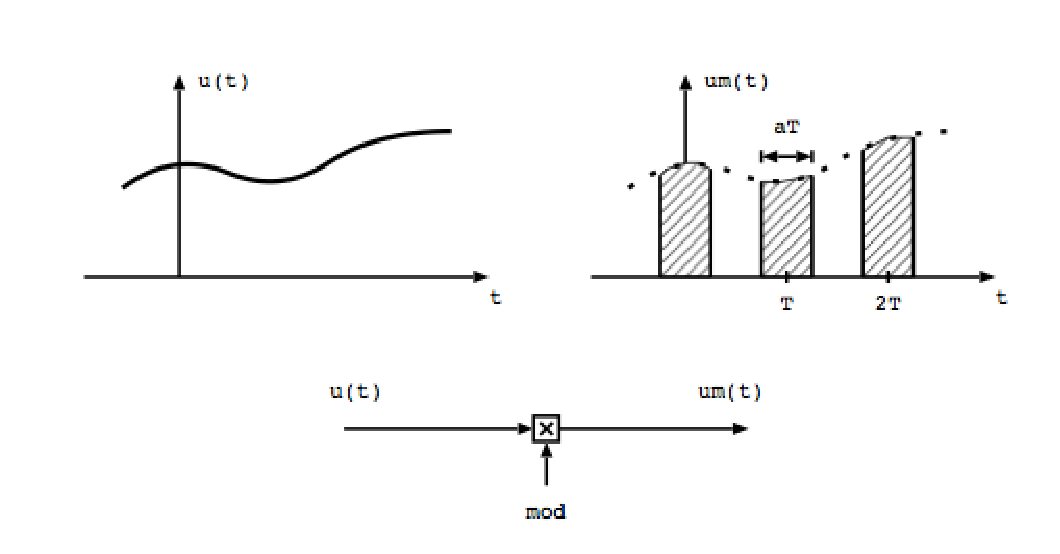
\includegraphics[scale=0.6, trim = 0cm 0cm 0cm 0cm, clip]{./Bilder/PrinzipSignalausblendung}
                \caption{Prinzip der Signalausblendung}
                \cite{PrinzipSignalausblendung}
        \end{figure}
    
        Praktisch lässt sich diese Art der Modulation durch einen Schalter
        realisieren, der jeweils nur kurzzeitig geschlossen wird.\vspace{1em}
        
        Das oben erwähnte $\alpha$ bezeichnet in diesem Fall das
        Tastverhältnis. Es beschreibt den Prozentsatz wie breit ein Rechteck in Verhältnis zur angegebenen halben 
        Periodendauer ist. Mit Hilfe dieses Wertes $\alpha$ lassen sich die Zeitfenster einstellen, 
        die ein Signal zur Verfügung haben soll. Sollen beispielsweise zwei Signale auf einem Kanal mit Hilfe 
        von Time-Devision Multiplexing übertragen werden, wird das $\alpha =
        \frac{1}{2}$ gewählt und jedes der Signale hat die Hälfte der Zeit auf dem Kanal. Sollen wiederum auf dem selben 
        Kanal $100$ verschiedene Signale übertragen werden wird $\alpha = \frac{1}{100}$ und jedes Signal hat
        $\frac{1}{100}$ der Zeit auf dem Kanal.\vspace{1em}
        
        Interessant ist, welche Auswirkung diese Art der Modulation auf das
        Frequenzspektrum des Originalsignals hat.
        Dazu betrachten wir das Zeitsignal und transformieren es in den Frequenzbereich.
        
            \begin{equation*}
                \begin{split}
                    f_m (t)   &= f(t) \cdot \sqcap_{\alpha T} (t) \ast \delta_T (t) \\
                    F_S (j\omega) &= \frac{1}{2\pi} F (j\omega) \ast \left [
                    \alpha T \cdot si \left( \frac{\omega \cdot \alpha T}{2} \right) \cdot \omega_T \cdot \delta_{\omega
                    T} (\omega) \right] \\
                    &= \frac{1}{2\pi} F (j\omega) \ast \left [
                    \alpha \frac{2 \pi}{\omega_T} \cdot si \left( \frac{\omega \cdot \alpha T}{2} \right) \cdot \omega_T
                    \cdot \delta_{\omega T} (\omega) \right] \\
                    &= \alpha \cdot F (j \omega) \ast \left ( si \left( \frac{\omega \cdot \alpha T}{2} \right)
                    \sum_{k=-\infty}^{\infty} \delta (\omega - k\omega_T) \right)\\
                    &= \alpha \cdot F (j \omega) \ast \left ( si \left( \frac{\omega \cdot \alpha \frac{2
                    \pi}{\omega_T}}{2} \right) \sum_{k=-\infty}^{\infty} \delta (\omega - k\omega_T) \right)\\
                    &= \alpha \cdot F (j \omega) \ast \left ( si \left( \frac{\omega \cdot \alpha \pi}{\omega_T}
                    \right) \sum_{k=-\infty}^{\infty} \delta (\omega - k\omega_T) \right)\\
                    &= \alpha \cdot F (j \omega) \ast \sum_{k=-\infty}^{\infty} (si(k \pi \alpha) \cdot \delta (\omega -
                    k\omega_T))\\
                    &= \alpha \cdot \sum_{k=-\infty}^{\infty} \left [ si(k \pi \alpha) \cdot F (j(\omega - k\omega_T))
                    \right]\\
                \end{split}
            \end{equation*}
            
        Als Sonderfall sollte außerdem noch das Basisband ($k = 0$) erwähnt werden:
        
       \begin{equation*}
        	\begin{split}
        		U_m (j\omega) = \alpha \cdot U(j\omega)
        	\end{split}
        \end{equation*}        
        
        Diese Fourier-Transformation verdeutlicht, dass das gesamte Amplitudenspektrum im Frequenzbereich um den Faktor
        $\alpha$ gedämpft wird. Außerdem werden alle Bänder mit $k > 0$
        zusätzlich um den Faktor $si(k \pi \alpha)$ gedämpft. Falls das Produkt $k \cdot \alpha$ eine ganze Zahl und somit 
        das Produkt innerhalb der $si()$ Funktion
        ein ganzzahliges Vielfaches von $\pi$ ergibt, wird dieses Frequenzband
        vollständig gedämpft. Die Amplituden eines einzelnen Frequenzbandes werden jedoch nicht unterschiedlich zueinander gedämpft.\\
        
        Die eben besprochenen Auswirkungen der Modulation auf das Amplitudenspekrum verdeutlicht auch das folgende Bild.
        
        \begin{figure}[H]
        \centering
            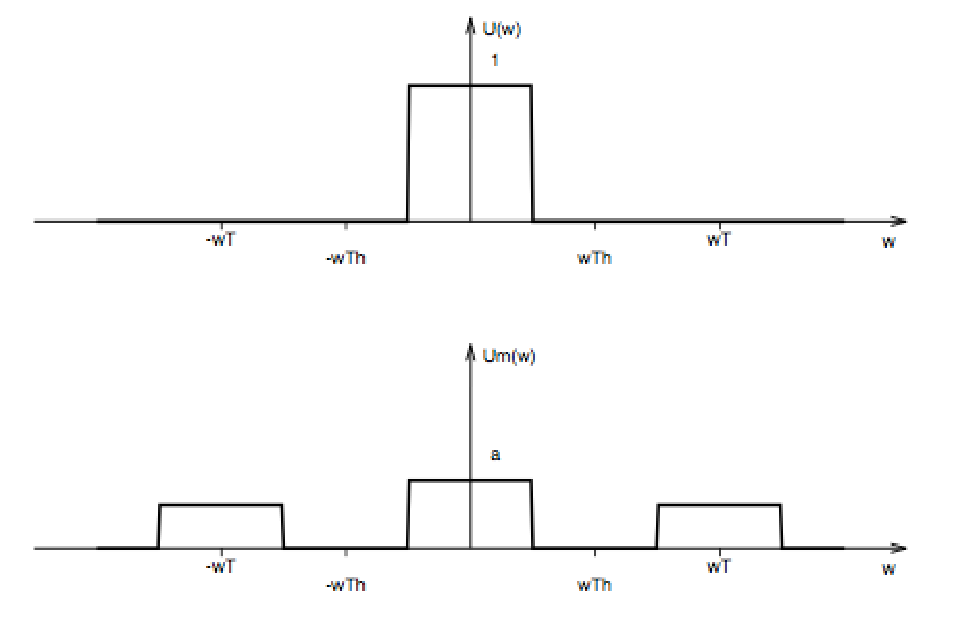
\includegraphics[scale=0.7, trim = 0cm 0cm 0cm 0cm, clip]{./Bilder/AmplitudenspektrumShap_Top}
                \caption{Amplitudenspektrum Shap-Top Sampling}
                \cite{AmplitudenspektrumShap_Top}
        \end{figure}
        
        Dieses Verhalten im Frequenzbereich ist ein großer Vorteil dieses Verfahrens der Pulsamplitudenmodulation. Die
        Amplitudenspektren werden zwar gedämpft, jedoch beiben sie unverzerrt.
        Diese Dämpfung lässt sich beim Empfänger wieder durch eine
        Verstärkung kompensieren. Problematisch wird es erst, wenn das $\alpha$ so klein wird, 
        dass die Amplituden des modulierten Signals auf die Größe der Rauschamplituden gedämpft werden.\vspace{1em}
        
        Da das modulierte Signal weiterhin wertekontinuerlich ist, lässt sich
        dieses Signal nur analog übertragen. Daher lassen sich auch keine Methoden der digitalen Verarbeitung anwenden, 
        wie beispielsweise die der Fehlererkennung. Dies ist ein entscheidender
        Nachteil dieses Verfahrens.\vspace{1em}
        
        Die Demodulation des Signals funktioniert auf die selbe Weise wie bei der Amplitudenmodulation. Das
        modulierte Signal wird tiefpassgefiltert. 
        
    \end{quote}%subsection
    
    \subsection{Abtastung mit Signalverbreiterung (flat-top sampling)}
    \begin{quote}
        Auch beim Flat-Top Sampling wird das Nutzsignal durch einen Schalter in bestimmte Zeitslots eingeteilt. Anders
        als beim Shape-Top sampling, bei dem als Dach des Rechtecks das Nutzsignal übertragen wurde, wird beim Flat Top
        Sampling der erste Wert des Nutzsignals zu Beginn eines Zeitslots über den gesamten Zeitslot übertragen. 
        Dazu wird zeitgleich zu dem Schalter auch noch ein Sample and Hold Glied
        geschaltet. Dieses Prinzip wird im folgenden Bild veranschaulicht.
        
        \begin{figure}[H]
        \centering
            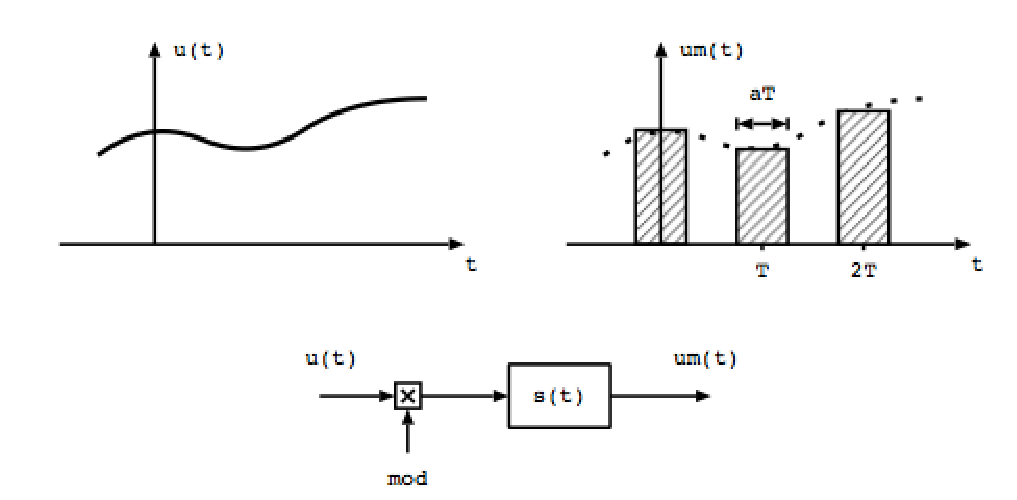
\includegraphics[scale=0.7, trim = 0cm 0cm 0cm 0cm, clip]{./Bilder/PrinzipSignalverbreiterung}
                \caption{Prinzip der Signalverbreiterung}
                \cite{AmplitudenspektrumShap_Top}
        \end{figure}
        
        Auch in diesem Fall ist ein Blick auf das Frequenzspektrum interessant.
        
            \begin{equation*}
                \begin{split}
                    f_m (t) &= [f (t) \cdot \delta_T (t)] \ast \sqcap_{\alpha T} (t)\\
                    F_F (j\omega) &= \left ( \frac{1}{2 \pi} F (j\omega) \ast \omega_T
                    \cdot \delta_T (\omega) \right) \cdot \alpha T \cdot si (\frac{\alpha \omega T}{2})\\
                    &= \alpha \cdot si \left( \frac{\omega \alpha T}{2} \right) \cdot \sum_{k=-\infty}^{\infty} F(j(\omega -
                    k\omega_T))\\
                    &= \alpha \cdot si \left( \frac{\omega \alpha \frac{2 \pi}{\omega_T}}{2} \right) \cdot
                    \sum_{k=-\infty}^{\infty} F(j(\omega - k\omega_T))\\
                    &= \alpha \cdot si \left( \frac{\omega \alpha \pi}{\omega_T} \right) \cdot
                    \sum_{k=-\infty}^{\infty} F(j(\omega - k\omega_T))\\
                \end{split}
            \end{equation*}

        Auch hier erwähnen wir den Sonderfall für das Basisband
        
        \begin{equation*}
        	\begin{split}
        		U_M (j\omega) = \alpha \cdot si \left( \frac{\omega \alpha \pi}{\omega_T}\right) \cdot U (j \omega)
        	\end{split}
        \end{equation*}
        
        Dieses Frequenzspektrum wird nicht nur um den Faktor $\alpha$ gedämpft,
        sondern zusätzlich auch noch um den Frequenzabhängigen Faktor $si \left( \frac{\omega \alpha \pi}{\omega_T}\right) $. 
        Diese Dämpfung erscheint auch schon in dem Basisfrequenzband und hat
        eine Verzerrung aller Frequenzbänder zur Konsequenz. Das Amplitudenspektrum sieht daher folgendermaßen aus:
        
        \begin{figure}[H]
        \centering
            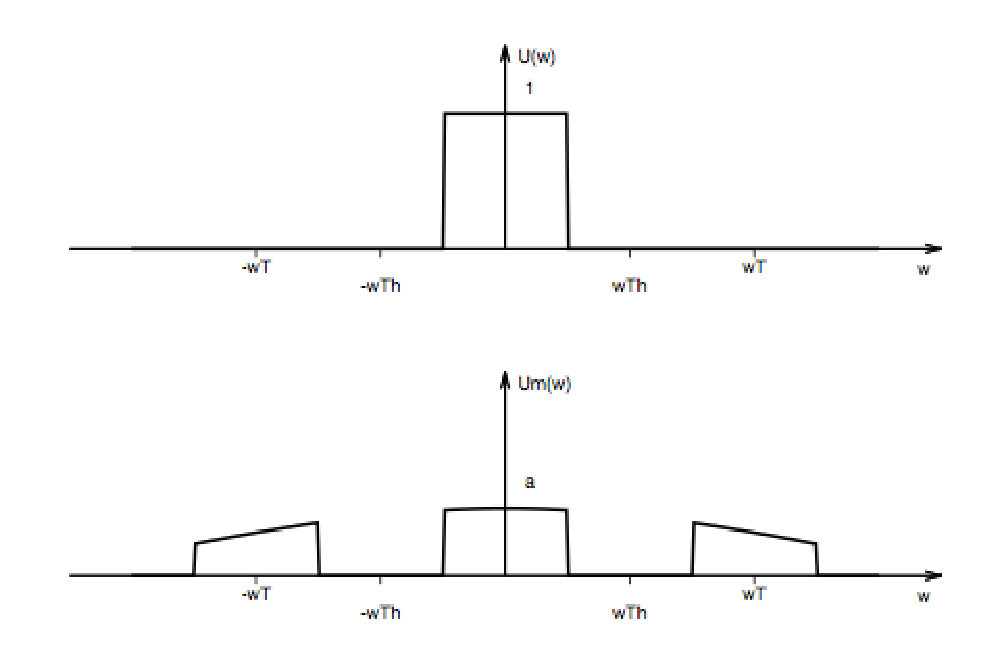
\includegraphics[scale=0.7, trim = 0cm 0cm 0cm 0cm,
            clip]{./Bilder/AmplitudenspektrumFlat_Top}
                \caption{Amplitudenspektrum Flat-Top}
                \cite{AmplitudenspektrumFlat_Top}
        \end{figure}
        
        Dieses verzerrte Spektrum lässt sich im Gegensatz zu dem Shape-Top gesampelten Signal nicht durch einen Teifpass
        wieder $100$ prozentig wiederherstellen. Das demodulierte Signal wird weiterhin verzerrt bleiben. Dies ist ein
        großer Nachteil des Flat-Top Sampling.\\
        Der Vorteil dieses Verfahrens ist es, dass das modulierte Signal sich als digitales Signal übertragen lässt und
        sich somit alle weiteren Verfahren der digitalen Übertragungstechnik anwenden lassen. 
    
	\end{quote}%subsection
\end{quote}%section

%--------------------------------------------------------------------
%--------------------------------------------------------------------    
\section{Vorbereitungsaufgabe}
\begin{quote}
    \subsection{Herleitung der Spektren}
    \begin{quote}
        Zunächst werden die Formeln für das Spektrum eines abgetasteten Signals
        hergeleitet. Das $\alpha$ steht dabei für das Tastverhältnis.\\
        Diese Herleitungen sind bereits ausführlich in der Theorie bearbeitet
        und können da eingesehen werden.
        
    \end{quote}  % Ende Subsection        
    \subsection{Skizzieren}
    \begin{quote}
                
        Danach werden die resultierenden Spektren $F_S (j\omega)$ und $F_F (j\omega)$
        für das Nutzsignal
        \begin{equation*}
        f(t) = A \cdot cos(\frac{\omega_T}{5}t)     
        \end{equation*}
		mit $\alpha = 0.5$ und $\omega_T = 20\pi kHz$ skizziert.
        
         \begin{figure}[H]
            \centering
                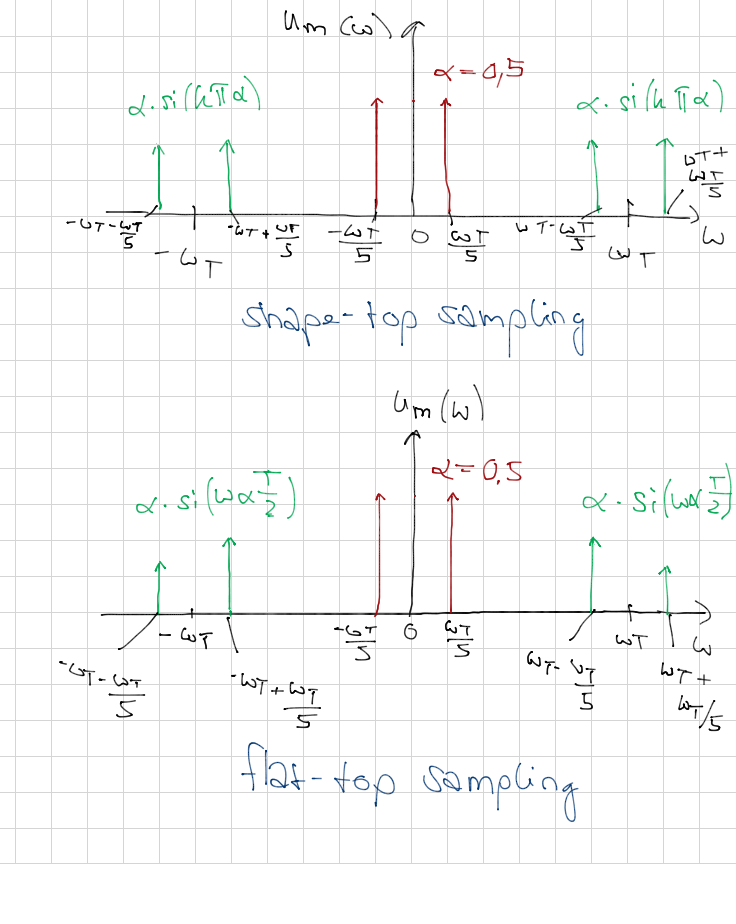
\includegraphics[scale=0.3, trim = 0cm 0cm 0cm 0cm,
                clip]{./Bilder/vorbereitungsskizze}
                    \caption{entstehende Spektren für shape-top und flat-top
                    sampling}
        \end{figure}
        
        Es ist zu sehen, dass sich die Amplituden der Spektren mit einem
        Si-Funktionsfaktor, welcher von dem eingesetzten $\alpha$ abhängt, verringern.
        Bei der shape-top Abtastung ist dieser Faktor unabhängig von der Frequenz
        $\omega$. Daher sind die Amplituden der Peaks, die an den Grenzen eines
        Frequenzbandes entstehen, immer gleich groß.        
        Bei der flat-top Abtastung ist dieser Faktor sogar von der Frequenz abhängig, daher entsteht 
        eine Amplitudenverringerung von zwei Peaks an den Rändern eines
        Frequenzbandes.\\
        Mit $\alpha$ gegen $0$ geht auch die Amplitude des Basisbands (k = $0$) gegen
        $0$. Somit werden alle folgenden Peakamplituden (deren Amplituden sich bei der
        shape-top Abtastung mit $\alpha \cdot si(k \pi \alpha)$ und bei der flat-top
        Abtastung mit $\alpha \cdot si(\frac{\omega \alpha T}{2})$ bilden) ebenfalls
        verschwindend gering. Ist das $\alpha$ aber $1$, beträgt die Amplitude des
        Basisbands $1$ und die folgenden Peakamplituden lassen sich wie bereits
        erwähnt berechnen.\\
        
        Interessant ist die Frage, an welchen Stellen sich diese Peaks auflösen,
        da eine si-Funktion bei einem Argument von einem Vielfachen von $\pi$
        den Wert null annimmt. Diese Überlegung kann man sowohl mithilfe des
        shape-top samplings, als auch anhand des flat-top-samplings lösen:\\
        
        Bei dem flat-top Verfahren angefangen, sieht man, wie erwähnt, dass die
        Amplituden der weiderholten Peaks im Spektrum mit dem Faktor 
        $\alpha \cdot si(\frac{\omega \alpha T}{2})$ abnehmen. Wenn man das
        Argument mit $T = \frac{2\pi}{\omega_T}$ umstellt, erhält man:
        
        \begin{equation*}
        	\begin{split}
        		si(\frac{\omega \alpha T}{2}) = si(\frac{\omega \alpha
        		2\pi}{2 \cdot \omega_T})
        	\end{split}
        \end{equation*}
        
        Für das gegebene $\alpha = 0.5$ und das $\omega_T = 20 \pi kHz$, muss
        das $\omega$ ein doppeltes Vielfaches der Abtastfrequenz sein. Mit
        $\omega = 2\omega_T$ oder $\omega = 4\omega_T$ usw. wird das Argument
        der si-Funktion zu einem ganzzahligen Vielfachen von $\pi$ und die Peaks
        im Spektrum an dieser Stelle der Frequenz heben sich auf.\\
        
        Das gleiche Ergebnis kann man feststellen, wenn man sich den jeweiligen
        Faktor bei der shape-top-Abtastung ansieht. Die Peakamplituden im
        Spektrum werden mit $\alpha \cdot si(k \pi \alpha)$ kleiner. Dies
        bedeutet, dass mit $\alpha = 0.5$ jede zweite Wiederholung der Peakpaare
        zu null werden. Da die Wiederholungen stets bei ganzen Vielfachen von
        $\omega_T$ auftreten, fällt auch hier jedes Peakpaar bei dem doppelten
        Vielfachen von $\omega_T$ weg.\\
        Bei einer breiteren Skizze des Spektrums, müsste auf diesen
        mathematischen Hintergrund Rücksicht genommen werden.
        
        
    \end{quote}  % Ende Subsection    
    
    \subsection{Planung und Durchführung}
    \begin{quote}
        Außerdem wird die Planung zur Praktikumsdurchführung im voraus gemacht. Für
        den Versuch haben wir uns folgendes überlegt.\\
        
        \begin{figure}[H]
            \centering
                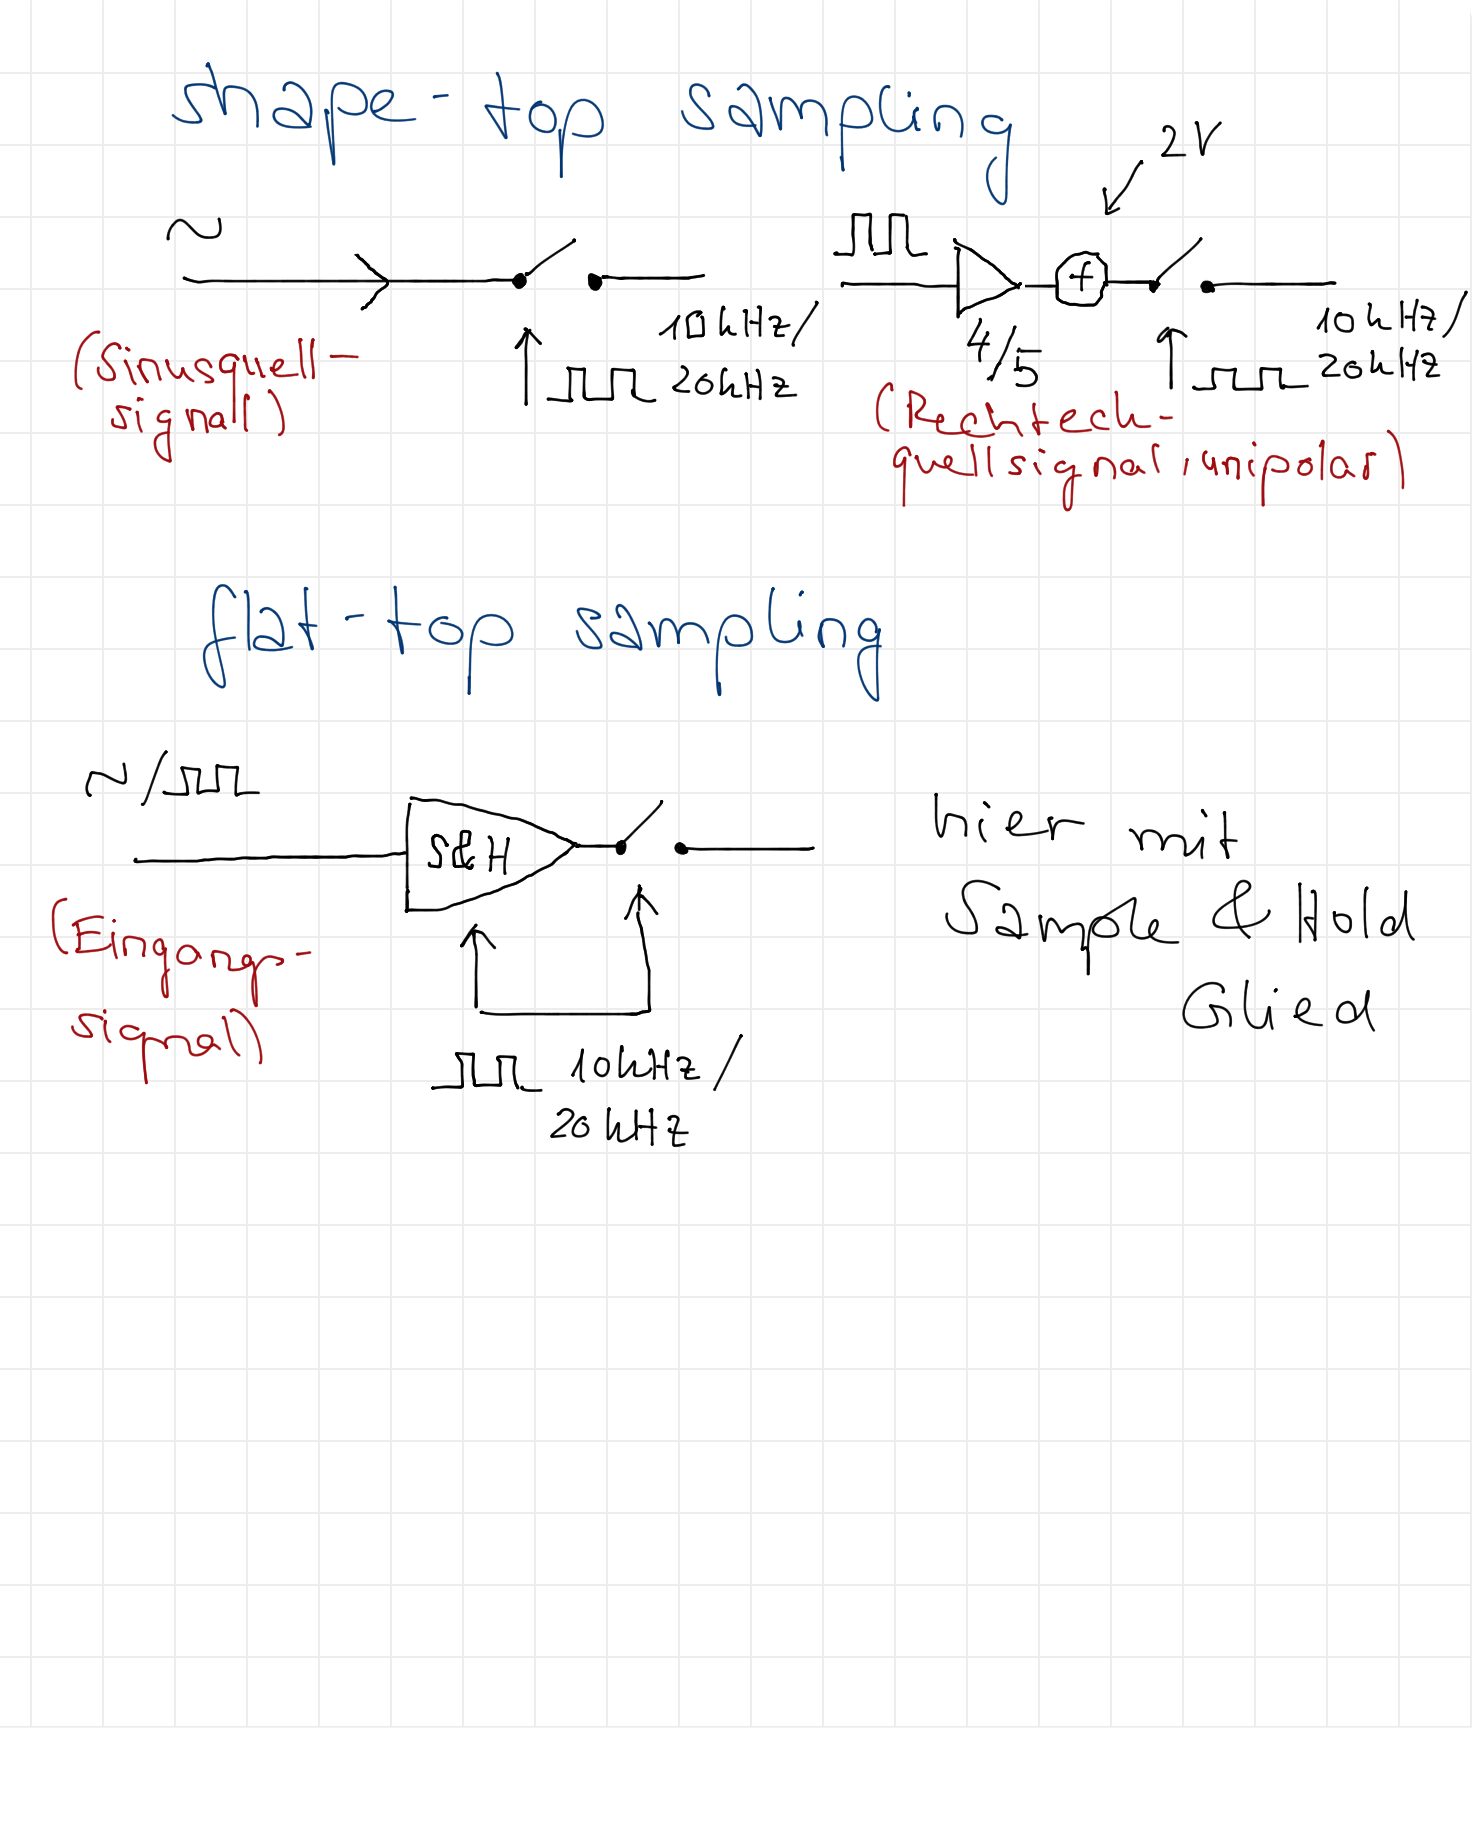
\includegraphics[scale=0.3, trim = 0cm 10cm 0cm 0cm,
                clip]{./Bilder/Blockschaltbilder.png}
                    \caption{Blockschaltbilder für den Versuchsaufbau der }
        \end{figure}
        
        Zuerst müssen die Quellsignale moduliert werden. Das Sinussignal
        kommt direkt aus dem Block Master Signals auf dem Steckbrett mit $2 kHz$ Fequenz und
        $2V$ Amplitude. An diesem Signal wird nichts verändert. Beim
        Rechtecksignal muss das Signal jedoch noch einmal gedämpft werden, da die Amplitude $5V$ und nicht die
        gewünschten $4V$ beträgt.
        Dazu verwenden wir den Addierer mit dem integrierten Dämpfer und
        reduzieren das Signal von $5V$ zuerst mit dem Faktor $\frac{4}{5}$ auf $4V$ und addieren dann $-2V$ drauf, um
        ein bipolares Rechtecksignal mit einer Peak-to-Peak Amplitude von $-2V$
        bis $+2V$ zu erhalten.\\
        Nun müssen diese Signale abgetastet werden:
        
        Für das shape-top sampling wird das Sinus-Quellsignal in den
        Schalter geführt, welcher über das Rechteck-Tastsignal mit $5V$ Amplitude und $10 kHz$ bzw. $20 kHz$
        Abtastfrequenz zustandsgesteuert ist. Durch den Schalter wird der Sinus
        entsprechend abgetastet und kann mithilfe des PicoScope grafisch
        dargestellt werden.\\ 
        Das modulierte Rechteckquellsignal wird ebenfalls in den
        zustandsgesteuerten Schlater geführt, wo es dann durch shape-top sampling
        abgetastet wird. 
        
        \vspace{0.5em}
        
        Für das flat-top sampling wird zusätzlich ein Sample and Hold Glied
        verwendet. Dieser befindet sich auf dem Steckbrett direkt über dem
        verwendeten Schalter und ist ebenfalls über das Rechtecktastsignal
        gesteuert. Beide Quellsignale werden hierbei zunächst in das Sample and
        Hold Glied geführt und aus dessen Ausgang in den Schalter
        weitergeleitet. So wird erst die zum Abtastzeitpunkt vorhandene
        Amplitude ermittelt und danach die Abtastung vollzogen. Das enstandene
        Signal kann anhand PicoScope grafisch mit dem Quellsignal ins Vergleich gesetzt
        werden.
        
    \end{quote}  % Ende Subsection	
    
    \subsection{Matlab-Simulation}
    \begin{quote}
    
        Zuletzt wird eine MATLAB-Simulation der Abtastung mittels Signalausblendung
        und Signalverbreiterung für ein Sinussignal als Quellsignal und der
        Abtastfrequenz von $400 kHz$ ausgeführt. Das verwendete Quellsignal
        hatte eine Amplitude von $2V$ und eine Frequenz von $2 kHz$. Das
        Abtastrechtecksignal hatte eine variable Frequenz ($10 kHz$ und $20 kHz$),
        eine Amplitude von $5V$ und ein
        variables Tastverhältnis von $0.2, 0.5$ oder $0.7$.\\
        
        Zuerst betrachten wir die Simmulationsergebnisse der Abtastung durch
        Signalausblendung:
        
         \begin{figure}[H]
        \centering
        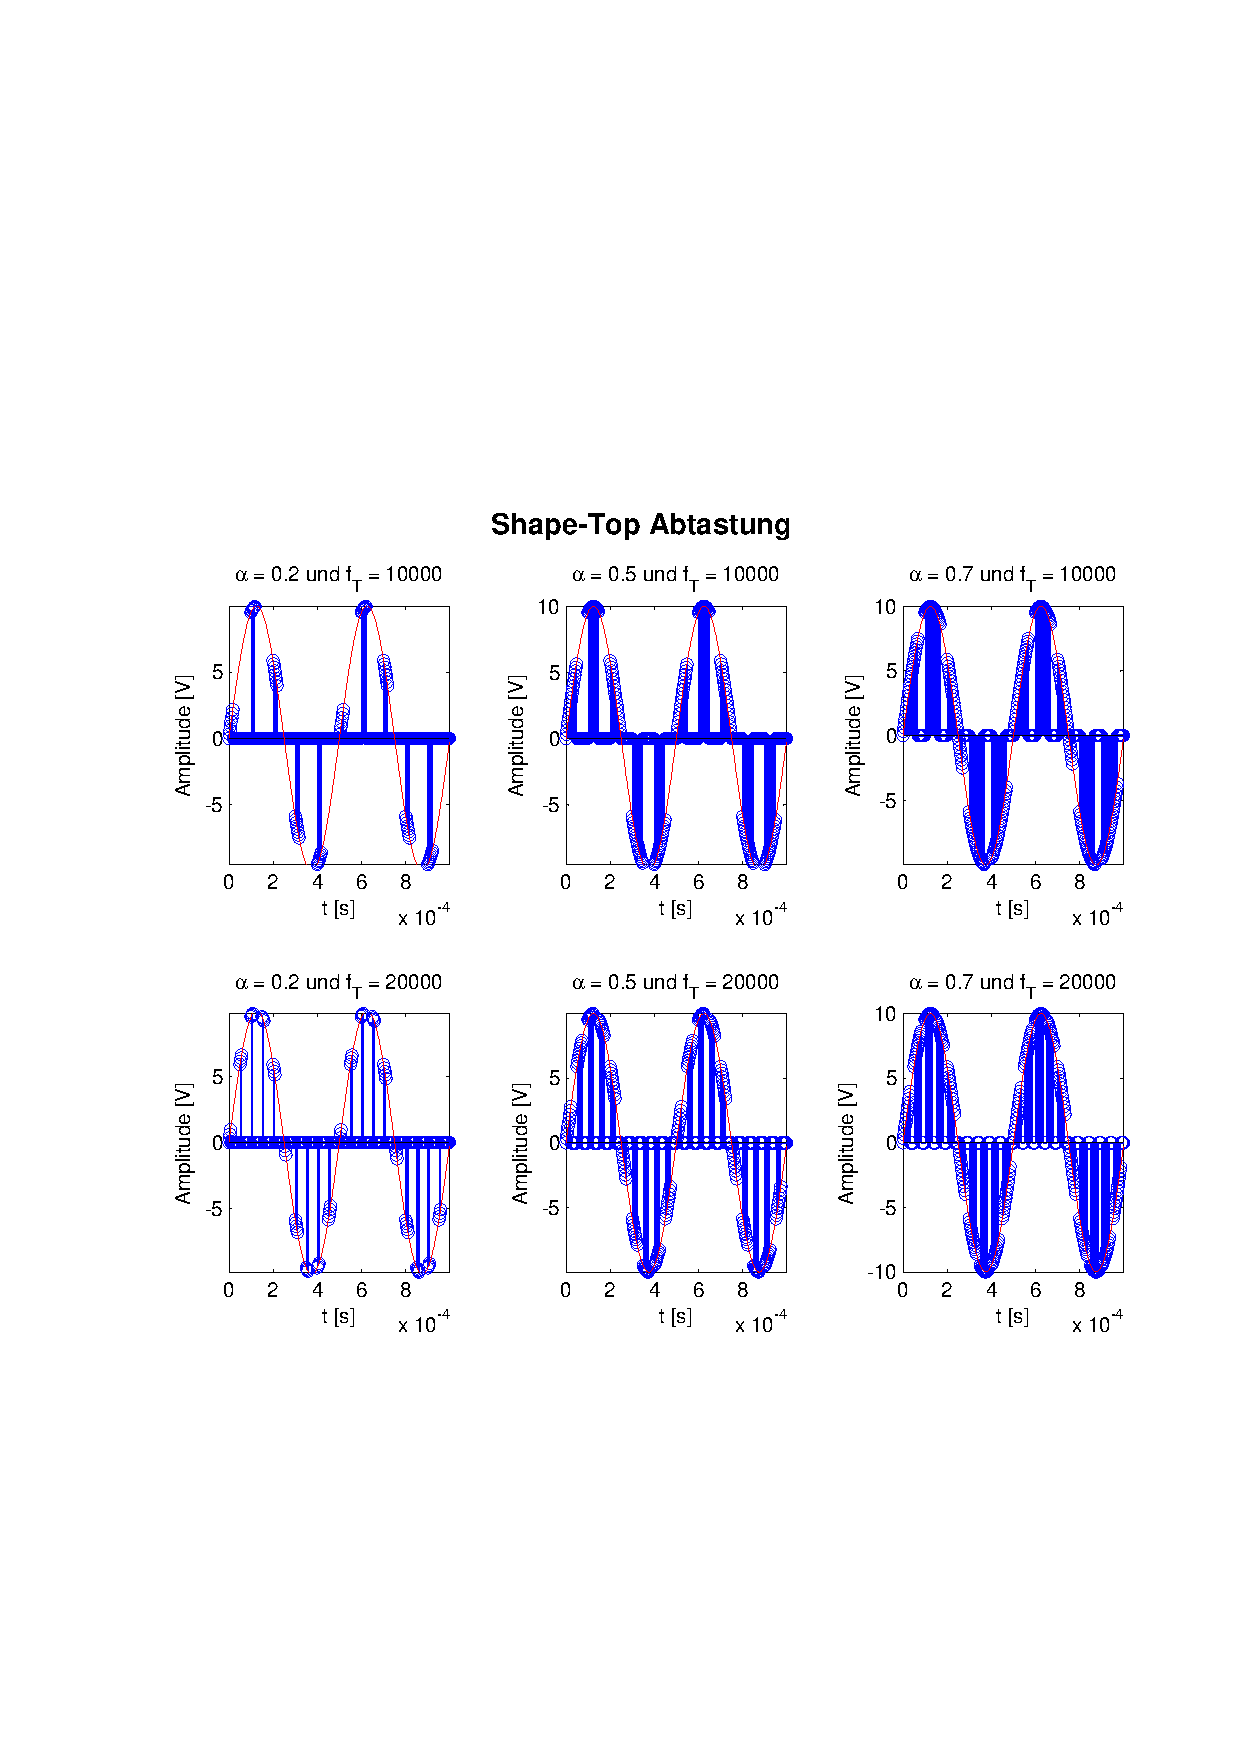
\includegraphics[scale=0.5, trim = 1.5cm 6cm 1cm 8cm,
        clip]{./Bilder/shape-top-zeit_5V}
            \caption{Zeitsignal mit shape-top-sampling}
  	    \end{figure}
  	    
  	    Im Zeitsignal sieht man eine maximale Amplitude von $10V$, welche durch
  	    die Multiplikation von den $2V$ des Quellsignals und dem $5V$ des
  	    Abtastsignals entsteht. Die Form der Rechtecke nehmen oben den
  	    Sinusverlauf des Quellsignals an, was im Zeitsignal den Unterschied zu
  	    der flat-top Abtastung ausmacht. Zusätzlich kann man deutlich sehen, dass
  	    die Verdopplung der Abtastfrequenz ungefähr doppelt so viele abgetastete Stellen ergibt und 
  	    dass ein größeres Tastverhältnis die Breite der Dauer der Abtastung erhöht. 
  	    Als Umhüllende haben wir das Quellsignal verwendet.\\
  	    
  	    \begin{figure}[H]
    \centering
        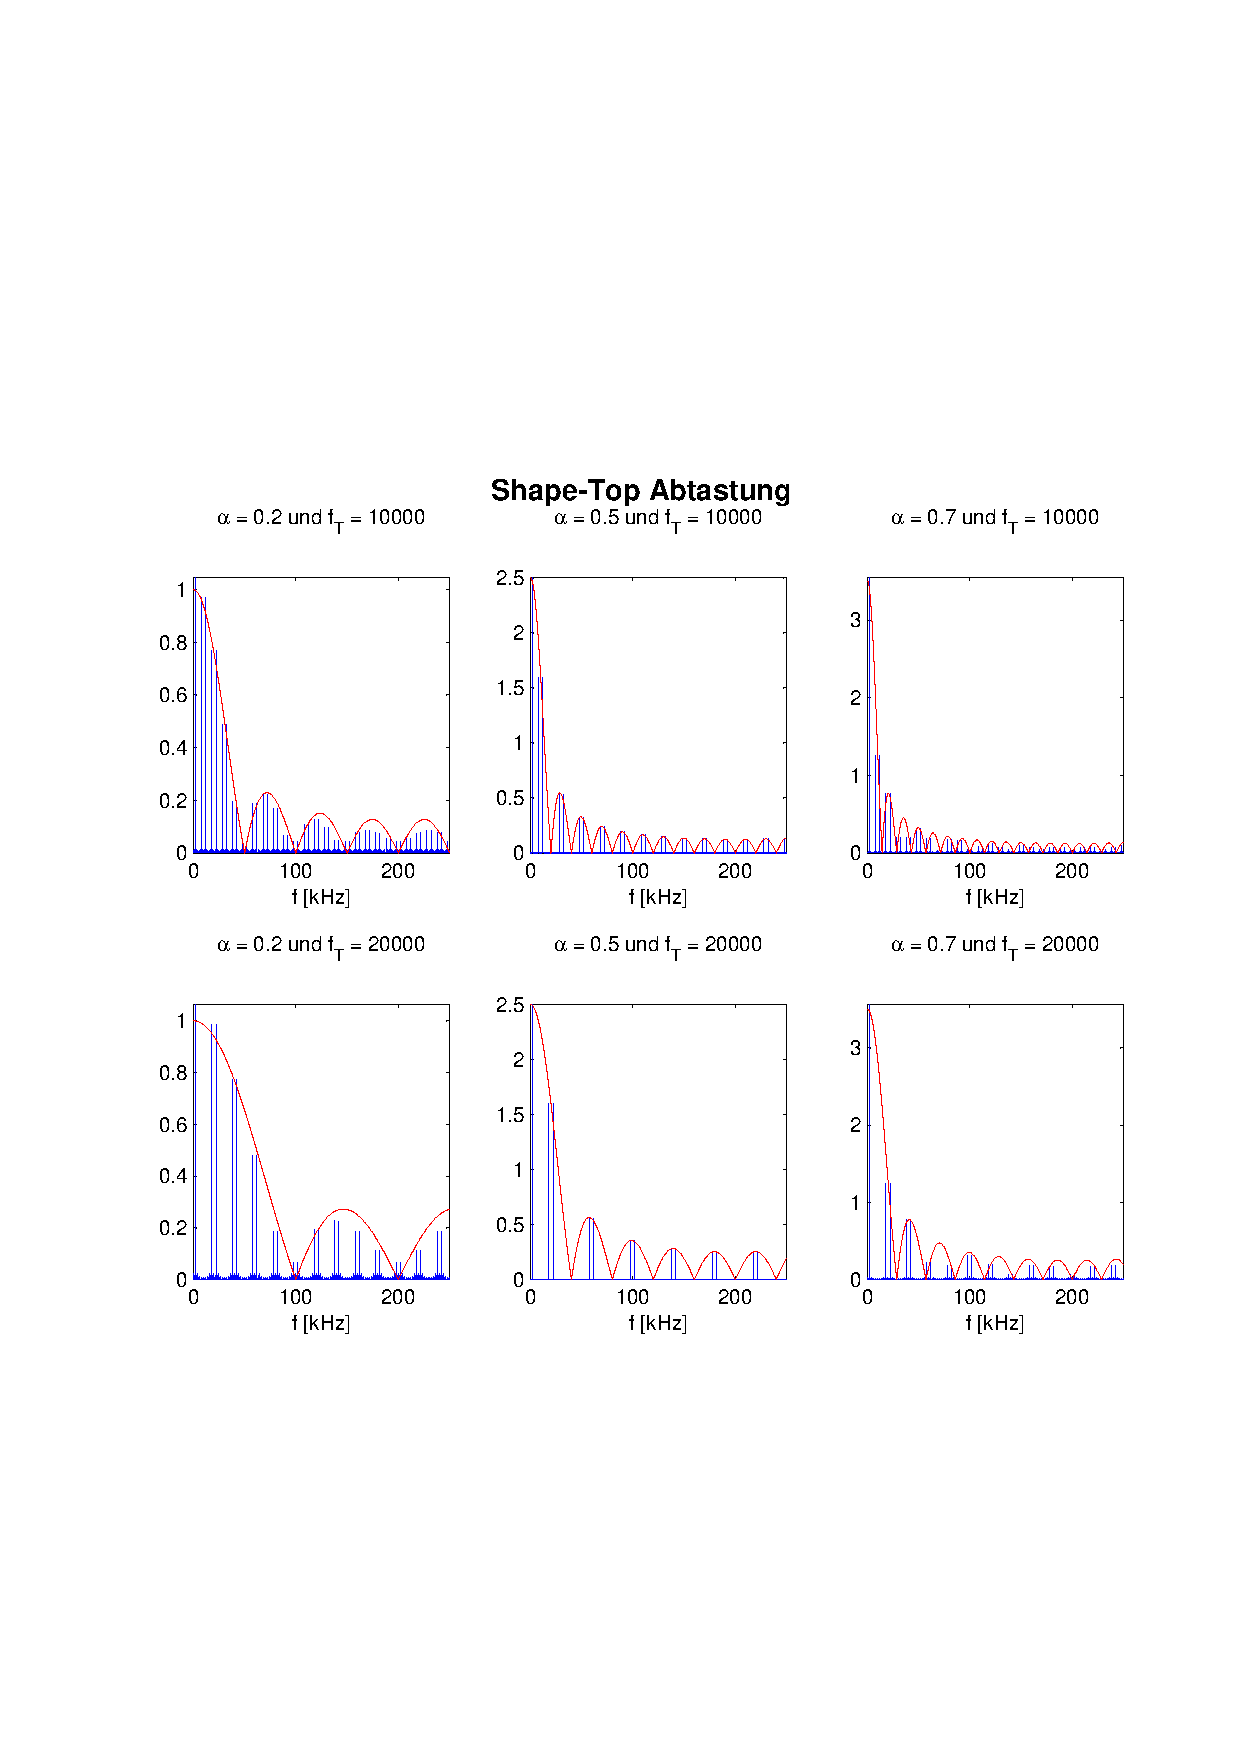
\includegraphics[scale=0.5, trim = 1.5cm 6cm 1cm 8cm,
        clip]{./Bilder/shae-top-freq_5V}
            \caption{Frequenzsignal mit shape-top-sampling}
  	    \end{figure}


  	    Im simulierten Spektrum kann man erkennen, dass die Amplituden der
  	    drei Basisbänder für die drei Tastverhältnisse exakt dem eingesetzten
  	    Tastverhältnis $\alpha$ mal $5V$ entsprechen. Mit wachsender Frequenz
  	    nehmen die Peaks deutlich an Amplitude ab. Außerdem kann man sehen, dass
  	    die auftretenden Peakpaare immer die gleiche Amplitude besitzen. Dieses
  	    unverzerrte Spektrum war bei einer shape-top Abtastung zu erwarten.
  	    Die Umhüllende des Spektrums ist eine Si-Funktion.
  	    \vspace{1em}
  	    
  	    Nun betrachten wir die Simulationsergebnisse der Abtastung mit
  	    Signalverbreiterung:
  	    
  	    \begin{figure}[H]
    \centering
        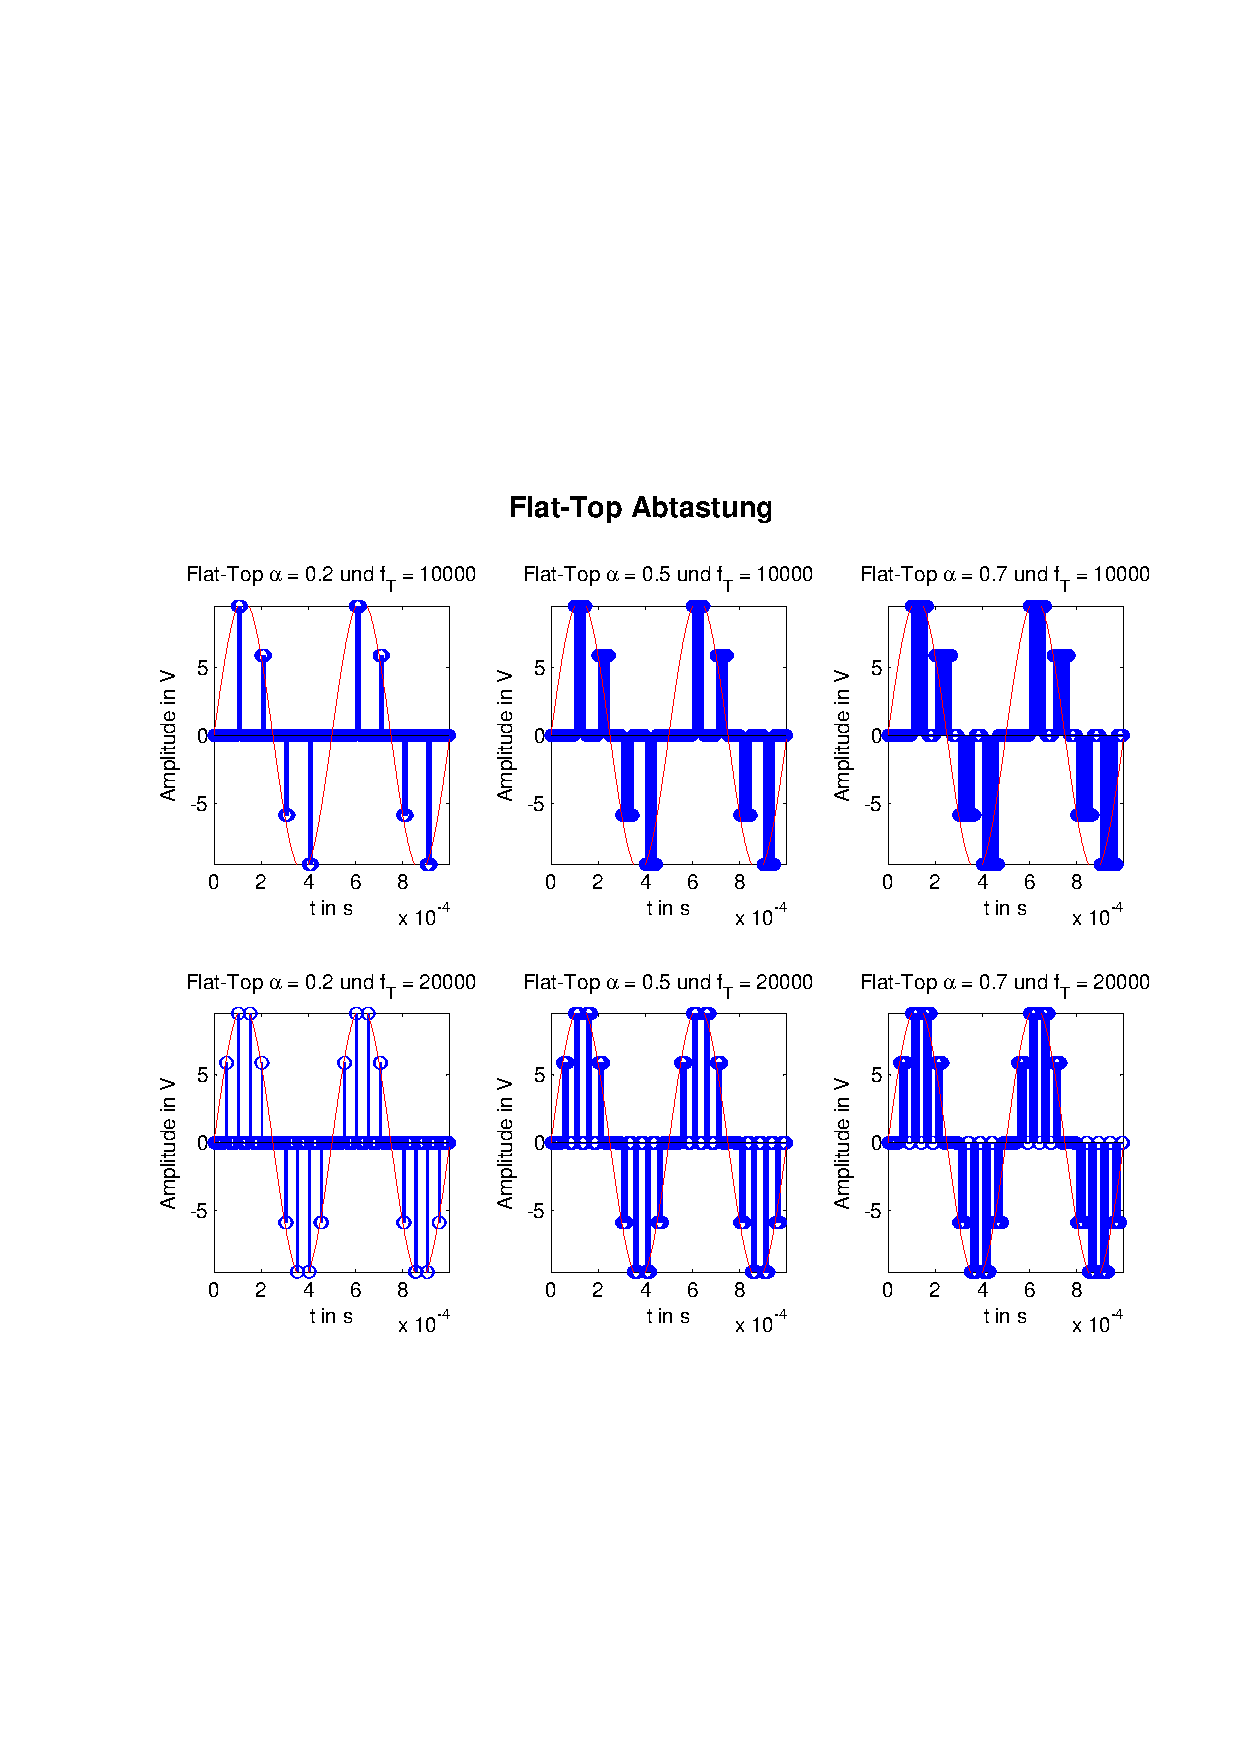
\includegraphics[scale=0.5, trim = 1.5cm 6cm 1cm 8cm,
        clip]{./Bilder/flat-top-zeit_5V}
            \caption{Zeitsignal mit flat-top-sampling}
  	    \end{figure}
  	    
  	    Die Amplituden, die Breiten und die Häufigkeiten der abgetasteten Stellen
  	    stimmen bei der flat-top Abtastung mit den Werten des Zeitsignals der
  	    shape-top Abtastung überein. Der einzige Unterschied, den man wie erwartet sehen
  	    kann, ist, dass die Rechtecke sich nicht dem Sinusverlauf anpassen
  	    sondern ab der Abtaststelle die Sinusamplitude annehmen und durch das
  	    Hold-Glied über die Dauer der Abtastung behalten. Daher sind diese
  	    Rechtecke oben flach.\\
  	    
  	    \begin{figure}[H]
    \centering
        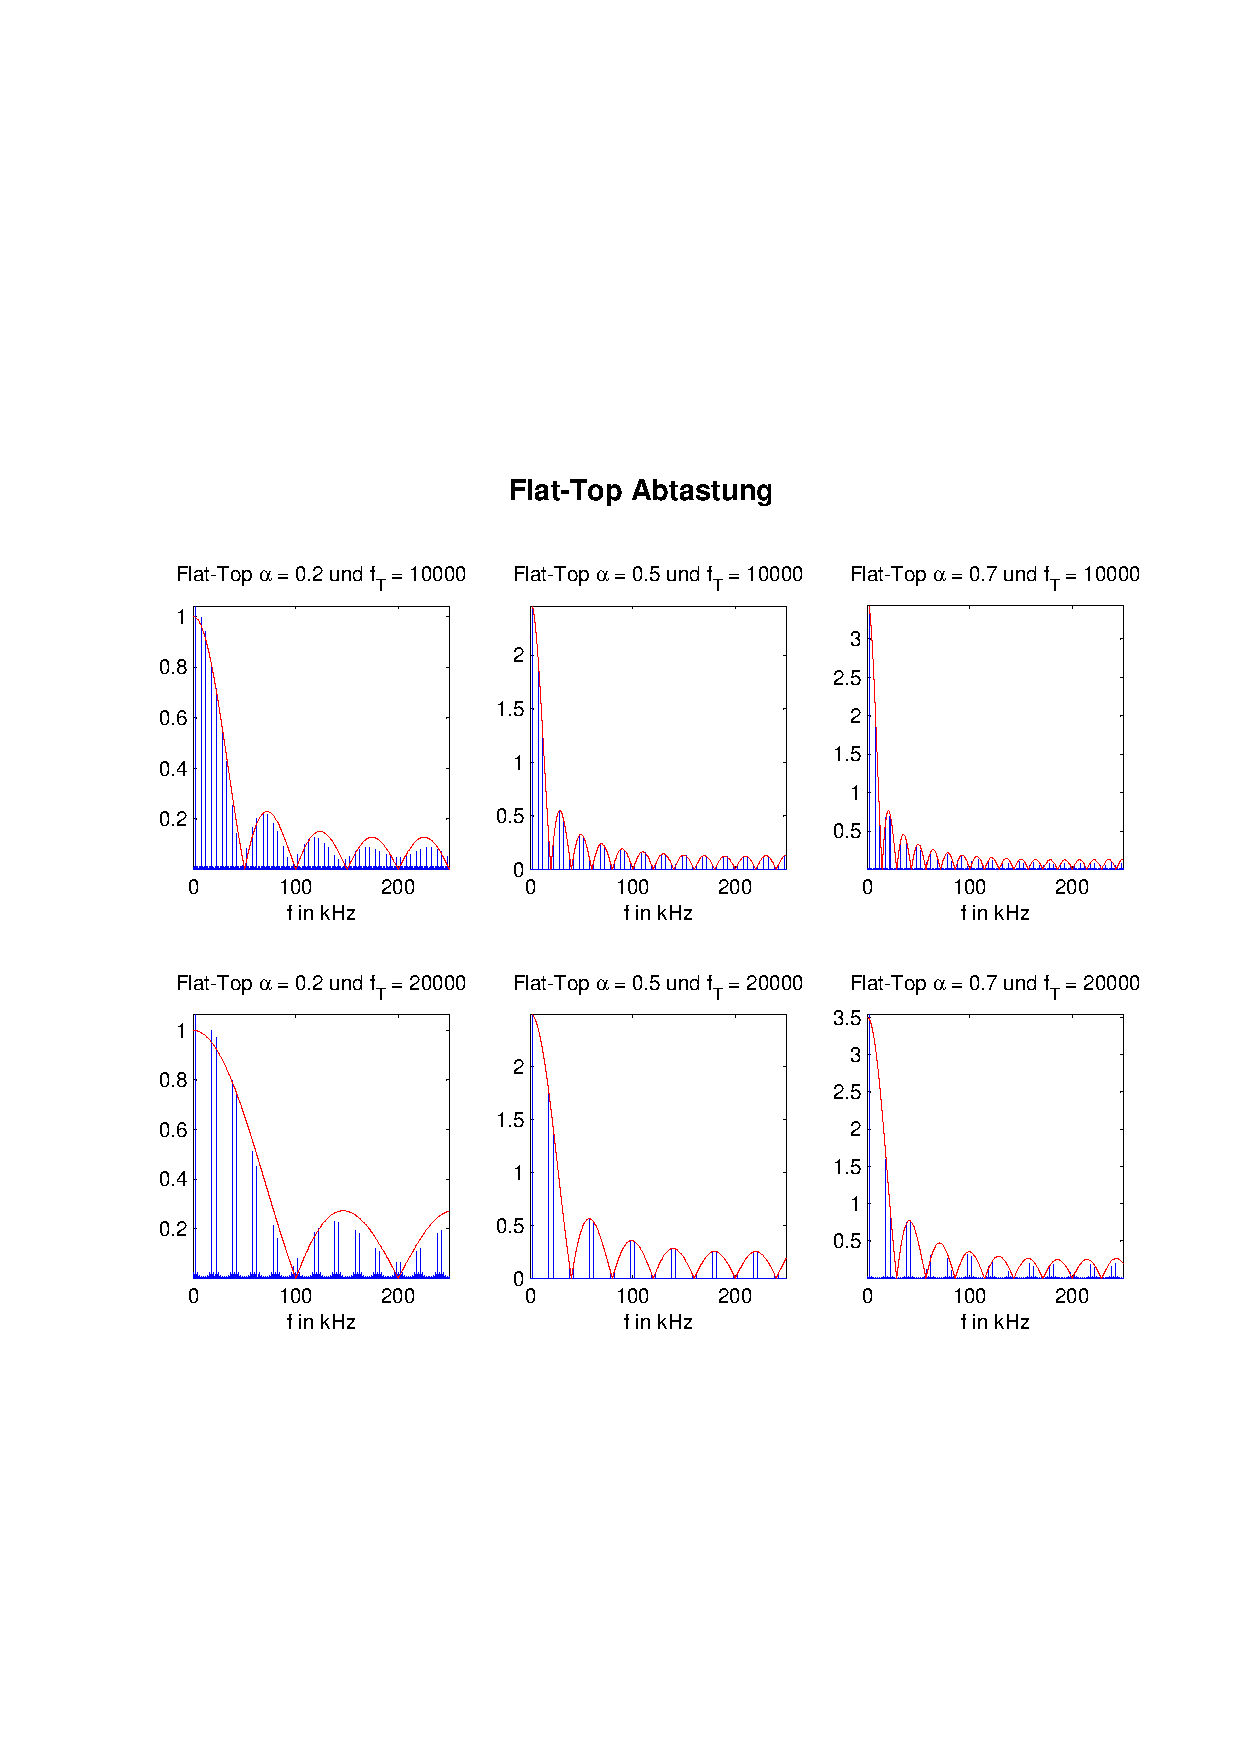
\includegraphics[scale=0.5, trim = 1.5cm 6cm 1cm 8cm,
        clip]{./Bilder/flat-top-freq_5V}
            \caption{Frequenzsignal mit shape-top-sampling}
  	    \end{figure}
  	    
  	    
  	    Durch die DFT dieser Rechtecke aus dem Zeitsignal entstehen in dem
  	    Spektrum Peaks mit frequenzabhängiger Amplitude, die deutlich
  	    besser in die umhüllende Si-Funktion passen, als das Spektrum einer
  	    shape-top Abtastung. Ansonsten verhält sich das Spektrum im Bezug auf
  	    Tastfrequenz und -verhältnis nicht anders als bei der Abtastung durch
  	    Signalausblendung.
        
    \end{quote}  % Ende Subsection	


\end{quote}%Theorie beenden

%--------------------------------------------------------------------
%--------------------------------------------------------------------    

    
    \section{Labordurchführung}
    \begin{quote}
         
         Nachdem wir die beiden realisierbaren, nichtidealen Abtastverfahren
         theoretisch realisiert haben, wurde nun die praktische Untersuchung
         dieser Verfahren der Pulsamplitudenmodulation zur Diskretisierung von
         zeitkontunierlichen Signalen durchgeführt. Dazu wurde, je nachdem
         welches Abtastverfahren untersucht werden sollte, eine
         Pulsamplitudenmodulationstrecke mit verschiedenen variablen Parametern
         entworfen und anhand dieser Strecke die Zeitsignale und die daraus
         entstehenden Spektren betrachtet.\\
         
         Als Abtastsignal verwendeten wir ein unipolares Rechtecksignal mit $5V$
         Amplitude und einer Abtastfreuquenz von entweder $10 kHz$ oder $20
         kHz$. Das Tastverhältnis wurde bei den Messungen zwischen $0.2$, $0.5$
         und $0.7$ abgewechselt. Dieses Abtastsignal erzeugten wir mithilfe des
         Signalgenerator und kontrollierten es vor jeder Messung mit dem
         Oszilloskop.\\
         
         Als Quellsignale wurden ein Sinus- und ein Rechtecksignal, sowie ein
         Rechtecksignal mit vorheriger RC-Tiefpassfilterung eingesetzt. Für den
         Sinus verwendeten wir den Block Master Signals auf dem Steckbrett, welcher uns, wie
         bereits in der Vorbereitungsaufgabe zum Versuchsaufbau erklärt, eine
         Amplitude von $2V$ und eine Frequenz von $2 kHz$ zur Verfügung
         stellte.\\
         Die Einrichtung des Rechteckquellsignals war etwas aufwendiger. Da das
         Steckbrett tatsächlich nur einen unipolaren Rechteck mit der Amplitude
         von $5V$ liefert, musste es erst auf das erwünschte bipolare Rechteck
         mit der Peak-to-Peak Spannung von $4V$ umgestellt werden. Dazu wird,
         wie ebenfalls vor dem Versuch erwartet, der Addierer mit der variablen
         Verstärkung zu Nutzen gezogen. Das Rechtecksignal wird vor der Addition
         mit einer Spannung von $-2V$, welche durch ein Rädchen an dem
         zweiten Summanden auf dem Addierer einstellbar ist, zunächst auf eine
         Spannung von $4V$ gebracht, in dem es mit dem Faktor $\frac{4}{5}$ gedämpft wird. 
         Die Dämpfung ist ebenfalls durch ein Rädchen einstellbar. Somit konnten
         wir das erwünschte Rechteckquellsignal für die Abtastung erstellen.\\
         Als letztes brauchten wir ein RC-tiefpassgefiltertes Rechtecksignal,
         welches ziemlich leicht zu realisieren war. Das zuvor erstellte
         Rechteck wurde vor der Abtastung durch einen RC-Filter auf dem
         Steckbrett geführt und konnte dann als drittes Quellsignal verwendet
         werden.\\
         
         Alle drei Quellsignale wurden mithilfe der Abtastung durch Signalausblendung und
         der Abtastung mit Signalverbreiterung abgetastet und auf ihre Spektren
         untersucht. Zusätzlich wurde duch eine Tiefpassfilterung des
         Ausgangssignals das jeweils verwendete Quellsignal rekonstruiert und
         mit dem abgetasteten Signal ins Verhältnis gesetzt. Die Ergebnisse,
         sowie die entstandenen Spektren sind in der Auswertung zu sehen.
         
         \vspace{1em}
         
         Nachdem die Abtastung dieser drei Quellsignale untersucht wurde,
         führten wir eine\\
         Sprachübertragung durch. Dazu wurde für ein beliebiges
         Sprachsignal ein shape-top und ein flat-top sampling realisiert und
         untersucht. Vorher wurde das Sprachsignal aber in den Summanden des
         Addierers mit variabler Verstärkung geführt, um um den Faktor $2$
         gedämpft zu werden. Wichtig bei dem versuch war es, dass das Mikrofon
         nicht zu nah an den verwendeten Lautsprechern (in unserem Fall
         Kopfhörer) stand, damit eine Rückkopplung vermieden werden konnte.
         Das Ergebis beider Abtastungen der Sprachübertragung ist ebenfalls in
         der Auswertung zu sehen.
         
   	\end{quote}%beende Labordurchführung

%--------------------------------------------------------------------
%--------------------------------------------------------------------    

    
    \section{Auswertung}
    \begin{quote}
    
        \subsection{Shape-Top Sampling}
        \begin{quote}    
        	Zuerst werden die Zeitbereiche eines shape-top abgetasteten
        	Sinusquellsignals betrachtet.
            
        	\begin{figure}[H]
            \centering
                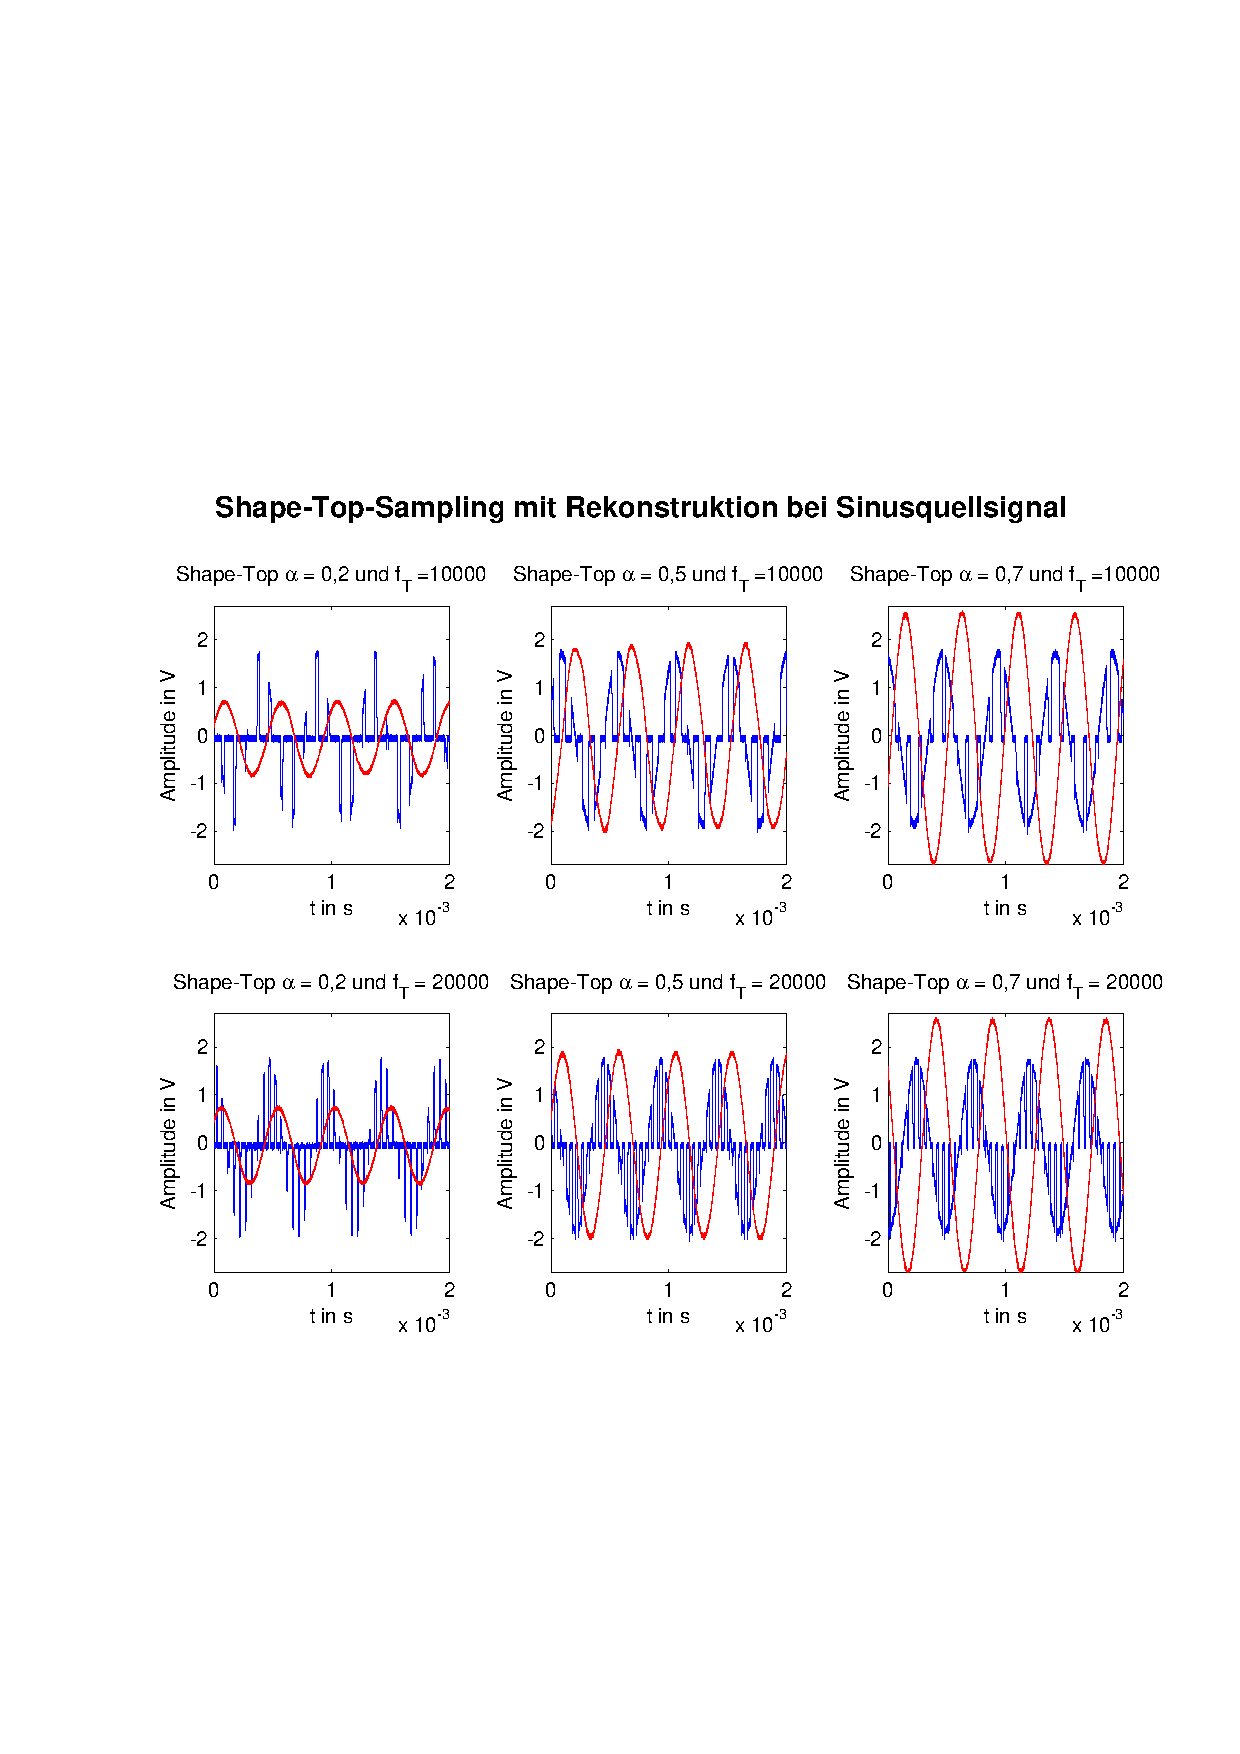
\includegraphics[scale=0.5, trim = 1.5cm 6cm 1cm 8cm,
                clip]{./Bilder/shape-top-sinus}
                    \caption{Zeitsignal einer shape-top-sampling mit Rekonstruktion
                    eines Sinusquellsignals}
          	\end{figure}
      	    
      	    Man kann sehen, dass mit wachsendem Tastverhältnis $\alpha$ die Breite
      	    der Abtastdauer zunimmt. Mit der doppelten Abtastfrequenz ist es
      	    sichtbar, dass mit der doppelten Häufigkeit abgetastet wird. Die
      	    rekonstruierten Signale konnten wir anhand eines Tiefpasses erstellen.
      	    Das abgetatstete Signal durchlief den Tiefpass auf dem Seckbrett,
      	    welcher ein einstellbares Gain besitzt. Je nachdem wie das Gain und die
      	    ebenfalls einstellbare Grenzfrequenzes auf dem Tiefpass eingestellt
      	    war, variierte die Amplitude und die Phase des rekonstruierten Signals.
      	    Da dies nicht der Schwerpunkt des Praktikums war, gaben wir uns damit
      	    zufrieden, wenn die Rekonstruktion einen erkennbaren Sinus wiedergab.\\
      	    
      	    
        	\begin{figure}[H]
            \centering
            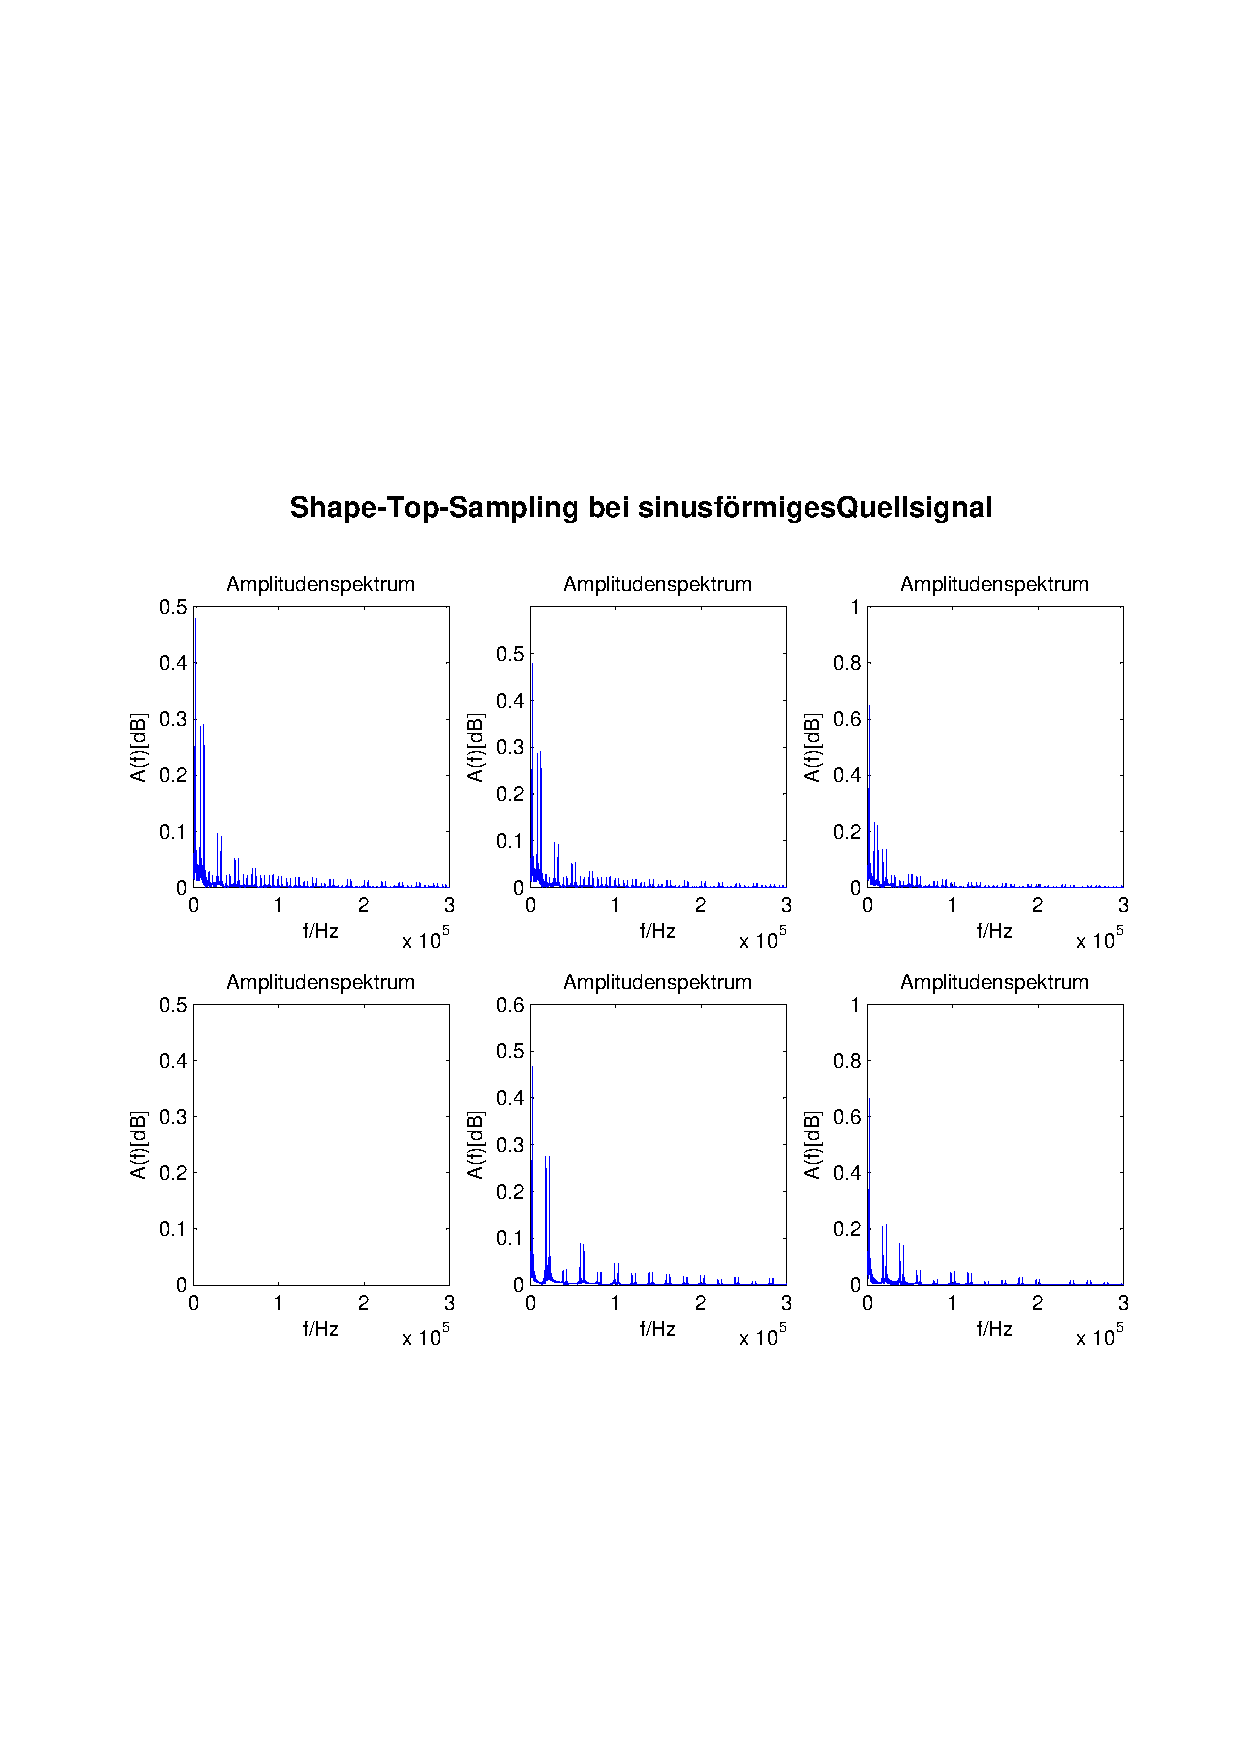
\includegraphics[scale=0.5, trim = 1.5cm 6cm 1cm 8cm,
            clip]{./Bilder/shape-top-sinus_freq}
                \caption{Frequenzsignal einer shape-top-sampling eines Sinusquellsignals}
      	    \end{figure}
      	    
            Die Frequenzspektren der Messsignale verhalten sich im großen und ganzen wie in der Theorie beschrieben und
            wie in der Vorbereitungsaufgabe schon mal geplottet. Es ist sehr schön zu erkennen, dass die Nebenbänder
            abfallen und auch wie erwartet auf einem Niveau bleiben.\\
            Leider hat der Datensatz des Sinus mit $\alpha = 0,2$ einen Fehler beim Erstellen des Spektrums ergeben.
            Daher fehlt dieses Spektrum. Die restliche $5$ Spektren verhalten sich jedoch wie erwartet.\vspace{1em}
            
            
                    
        	Bei dem Rechteckquellsignal ist ein ähnliches Ergebnis zu sehen, wobei die
        	Oberseite des Abtastrechtecks des shape-top-samplings bei einem Rechteck
        	nicht anders aussieht, als bei einem flat-top-sampling. Hier ist das
        	Zeitsignal:
        	   	
        	\begin{figure}[H]
            \centering
            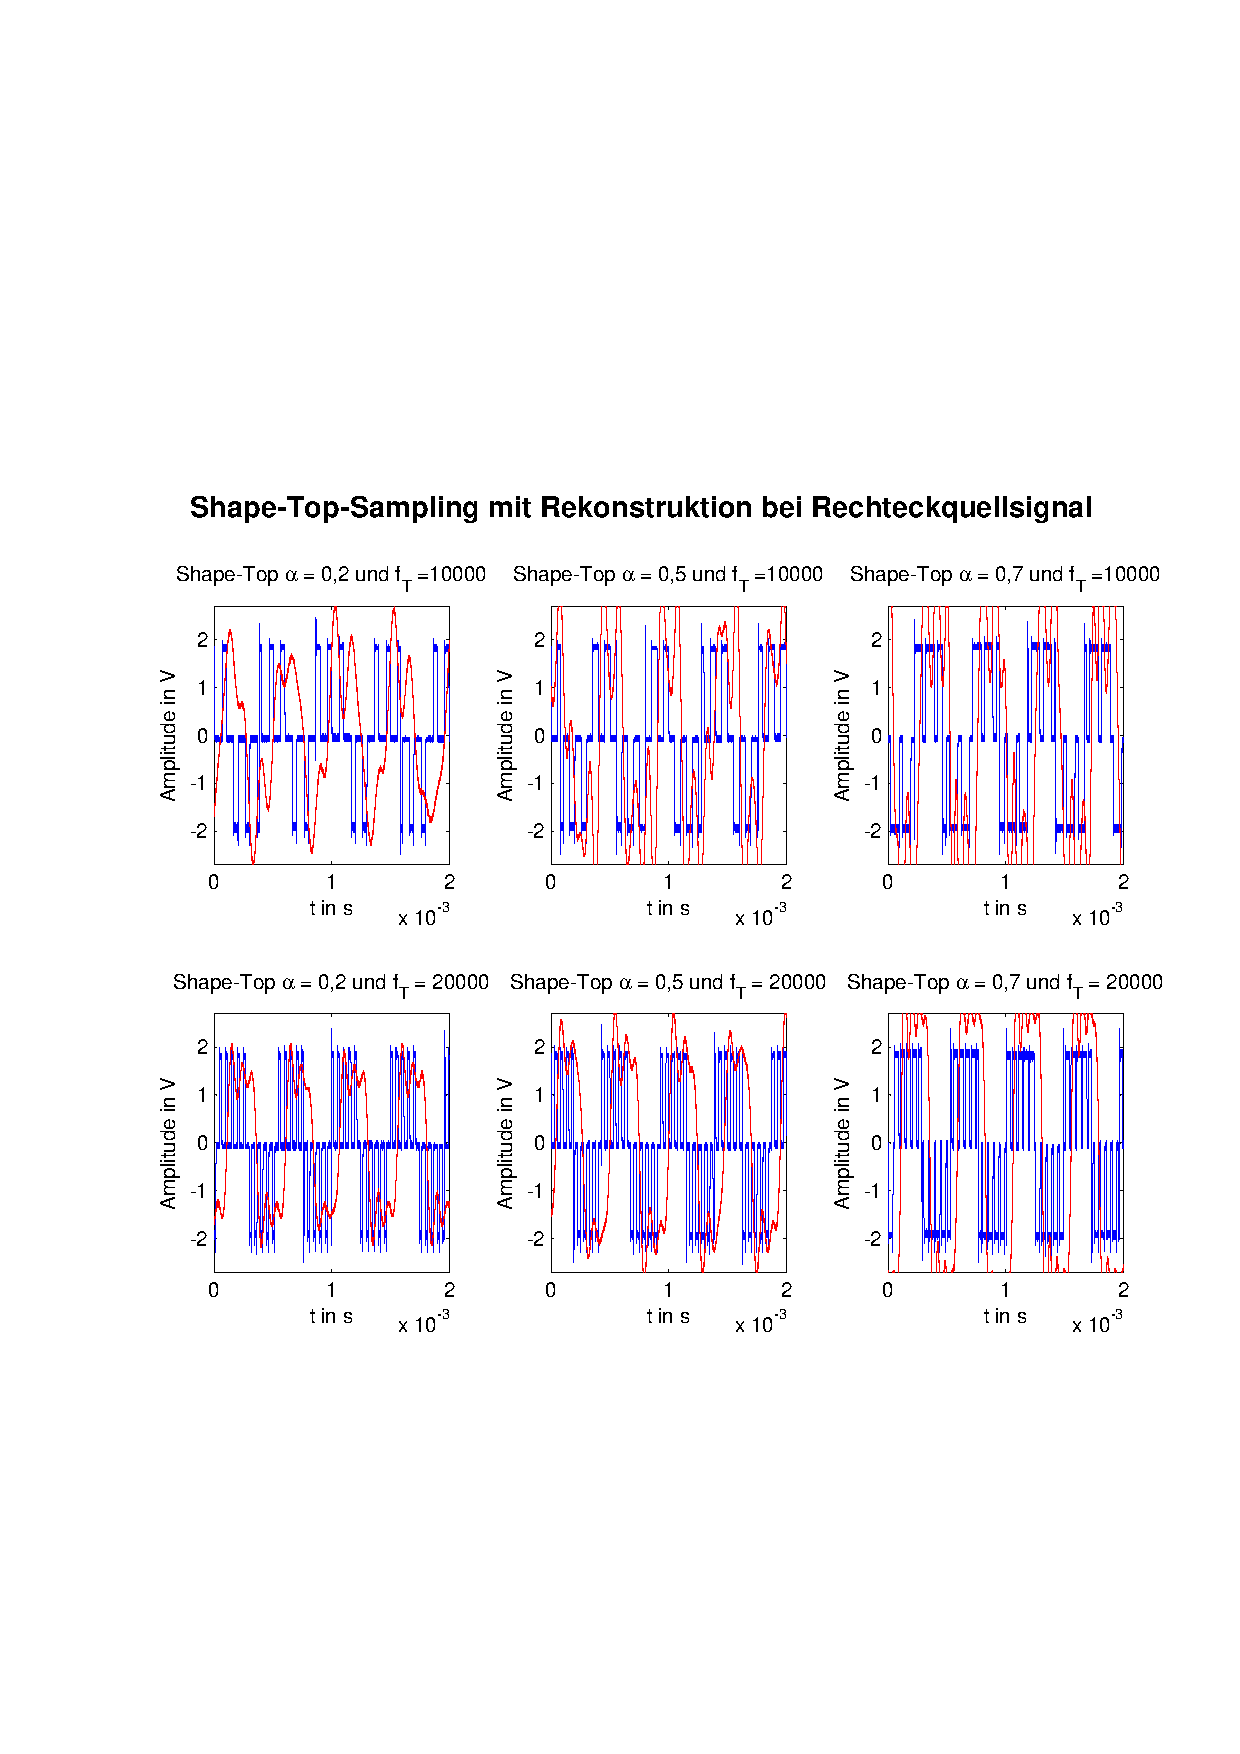
\includegraphics[scale=0.5, trim = 1.5cm 6cm 1cm 8cm,
            clip]{./Bilder/shape-top-recht}
                \caption{Zeitsignal einer shape-top-sampling mit Rekonstruktion
                eines Rechteckquellsignals}
      	    \end{figure}
      	    
      	    Die Eigenschaften bei erhöhtem Tastverhältnis und der doppelten
      	    Abtastfrequenz bleiben wie erwartet. Es ist deutlich erkennbar, dass
      	    die rekonstruierten Signale bei der Abtastfrequenz von $10 kHZ$ nicht
      	    einen sehr klar sichtbaren Rechteck wiedergeben. Dies ändert sich bei
      	    einer Abtastfrequenz von $20 kHz$. Dies liegt daran, dass die $10 kHZ$
      	    nicht der doppelten Bandbreite des Signals entspricht, welche ungefähr
      	    $8 kHz$ betrug. Dadurch können sich die periodischen Erweiterungen
      	    im Frequenzbereich überlagern und es entsteht Aliasing, welcher im
      	    Nachhinein nicht mehr korrigierbar ist. Tasten wir aber mit $20 kHZ$
      	    ab, ist die Abtastfrequenz mehr als doppelt so groß wie die Bangbreite
      	    des Signals und Aliasing kann ausgeschlossen werden. Dadurch werden die
      	    Rekonstruktionen, später auch bei dem Tiefpassgefiltertem
      	    Rechtecksignal, deutlich erkennbarer und unverzerrter als die
      	    Rekonstruktionen der mit $10 kHZ$ abgetasteten Signalen.\\
      	    
      	    Nun wird auch ein Frequenzgang dieses Rechtecksignals erstellt:
        	
        	
        	\begin{figure}[H]
            \centering
            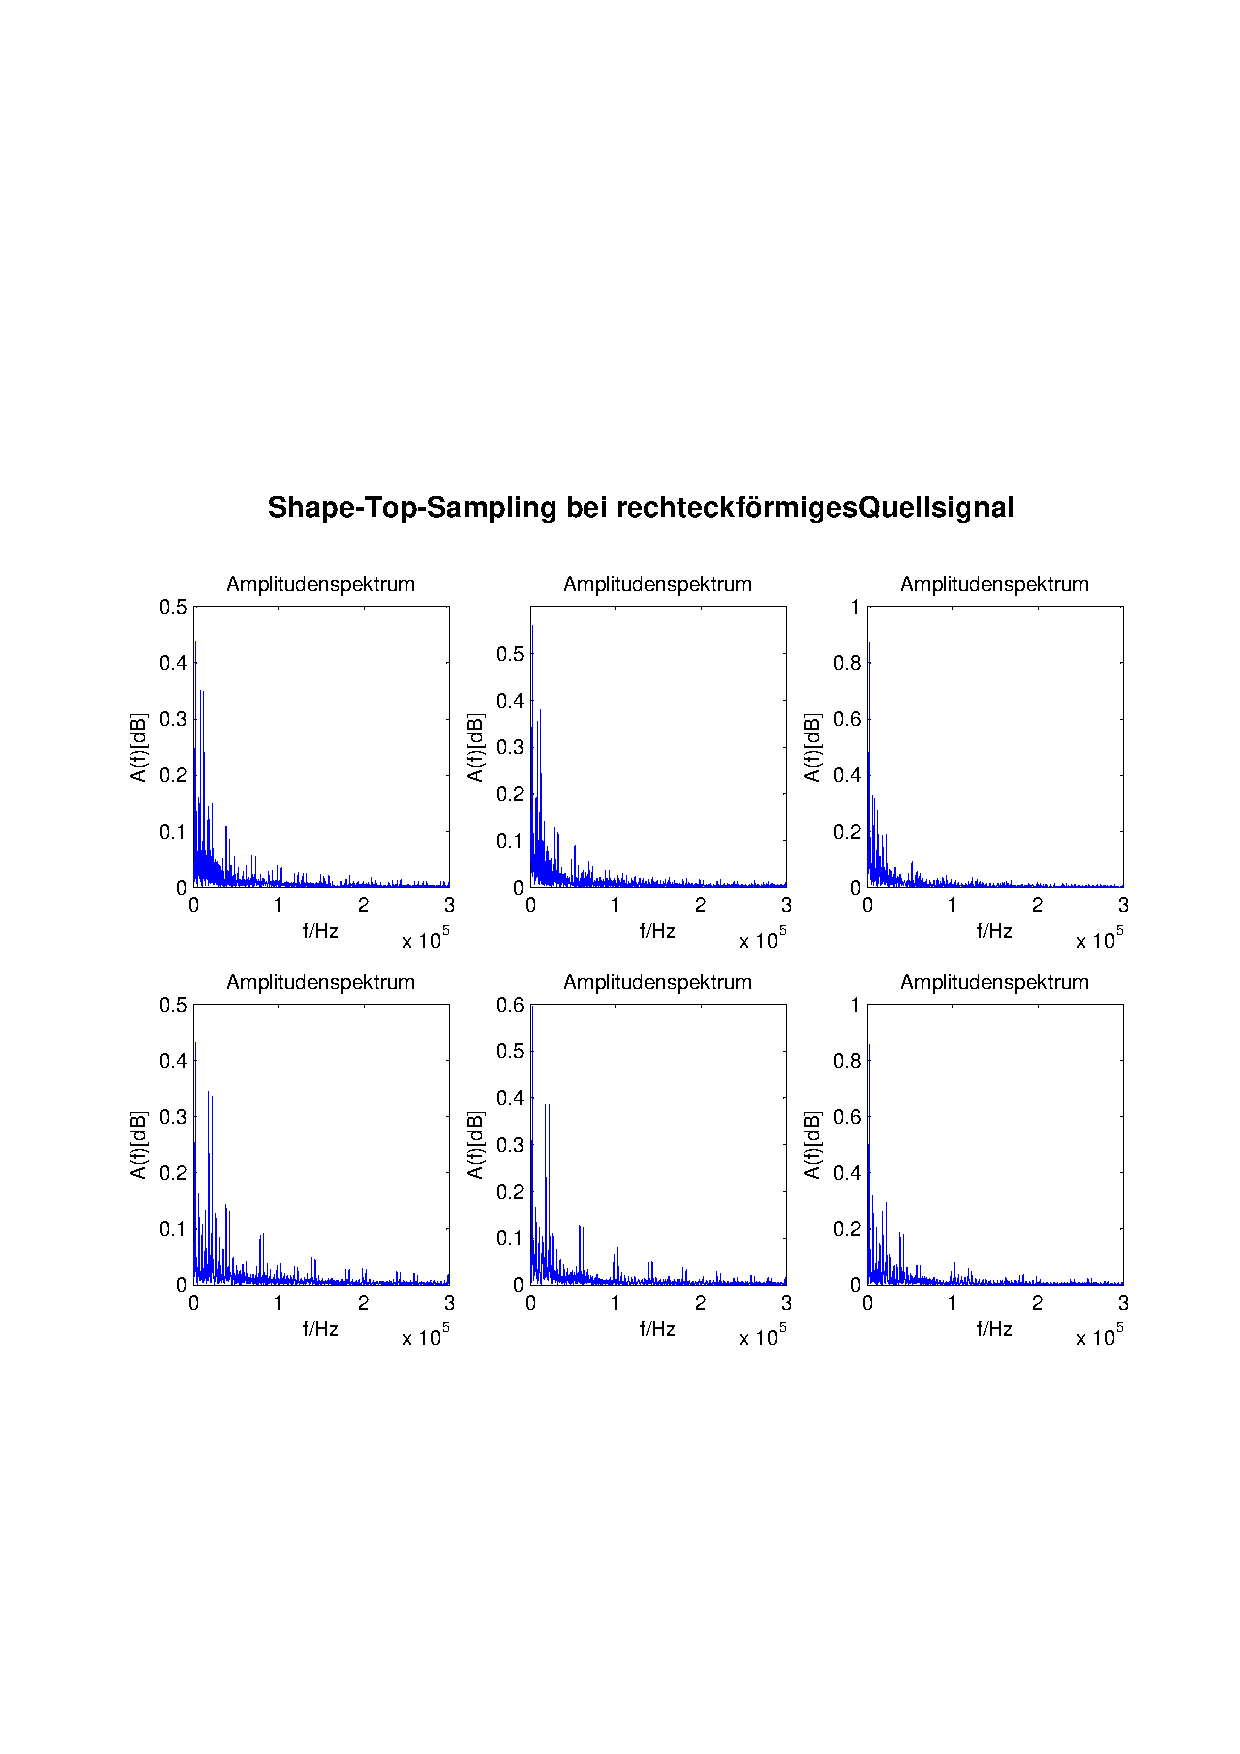
\includegraphics[scale=0.5, trim = 1.5cm 6cm 1cm 8cm,
            clip]{./Bilder/shape-top-recht_freq}
                \caption{Frequenzsignal einer shape-top-sampling eines Rechteckquellsignals}
      	    \end{figure}
      	    
        	Es ist erkennbar, dass das Spektrum grob eine si-Funktion darstellt.
			Dennoch ist es nicht genau erkennbar, da die Peakpaare, die durch die
			periodische Wiederholung entstehen, stets die gleiche Amplitude besitzen, was
			das komplette Spektrum nicht ganz der erwarteten si-Funktion entsprechen
			lässt. Dennoch sind wir mit dem Ergebnis zufrieden.\\
        
        
        	Zuletzt werden die Zeit- und die Frequenzbereiche des tiefpassgefilterten
        	Rechtecks betrachtet. Zuerst der Zeitbereich:
        	
        	\begin{figure}[H]
            \centering
            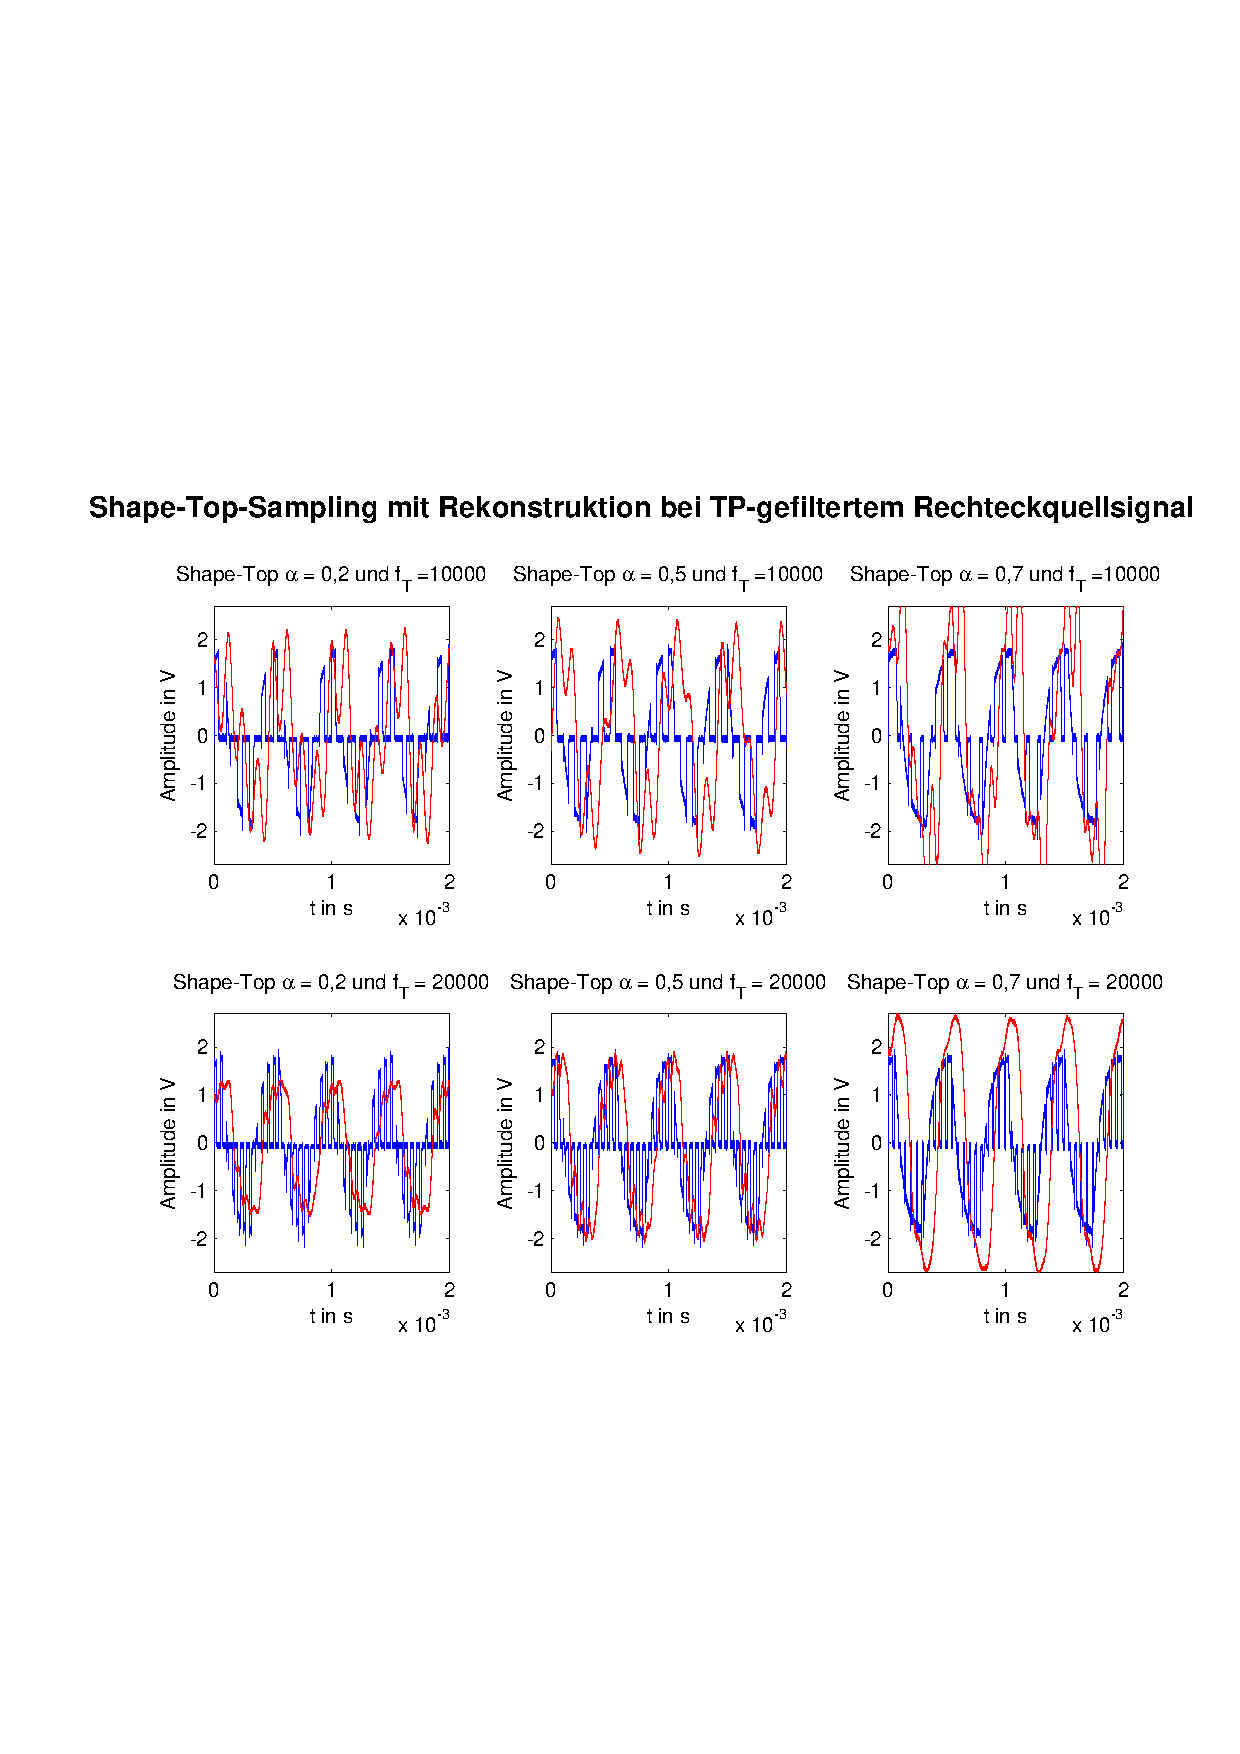
\includegraphics[scale=0.5, trim = 1.5cm 6cm 1cm 8cm,
            clip]{./Bilder/shape-top-tp-recht}
                \caption{Zeitsignal einer shape-top-sampling mit Rekonstruktion
                eines tiefpassgefilterten Rechteckquellsignals}
      	    \end{figure}
        	 
        	Das tiefpassgefilterte Rechtecksignal verläuft rundlich, man kann ein
        	urspüngliches Rechteck kaum wieder erkennen. Dennoch passt sich die obere Seite des
        	Abtastrechtecks der Form des Quellsignals an. Wieder bleiben die erwarteten
        	Eigenschaften bei verändertem $\alpha$ und veränderter Abtastfrequenz
        	erhalten und die Rekonstruktionen sind bei einer Abtastung mit $20 kHZ$ aus
        	dem bereits erwähntem Grund viel deutlicher als gefiltertes Rechteck zu
        	erkennen.\\ 
        	
        	Im Frequenzbereich sieht die Abtastung folgendermaßen aus:
        	
        	\begin{figure}[H]
            \centering
            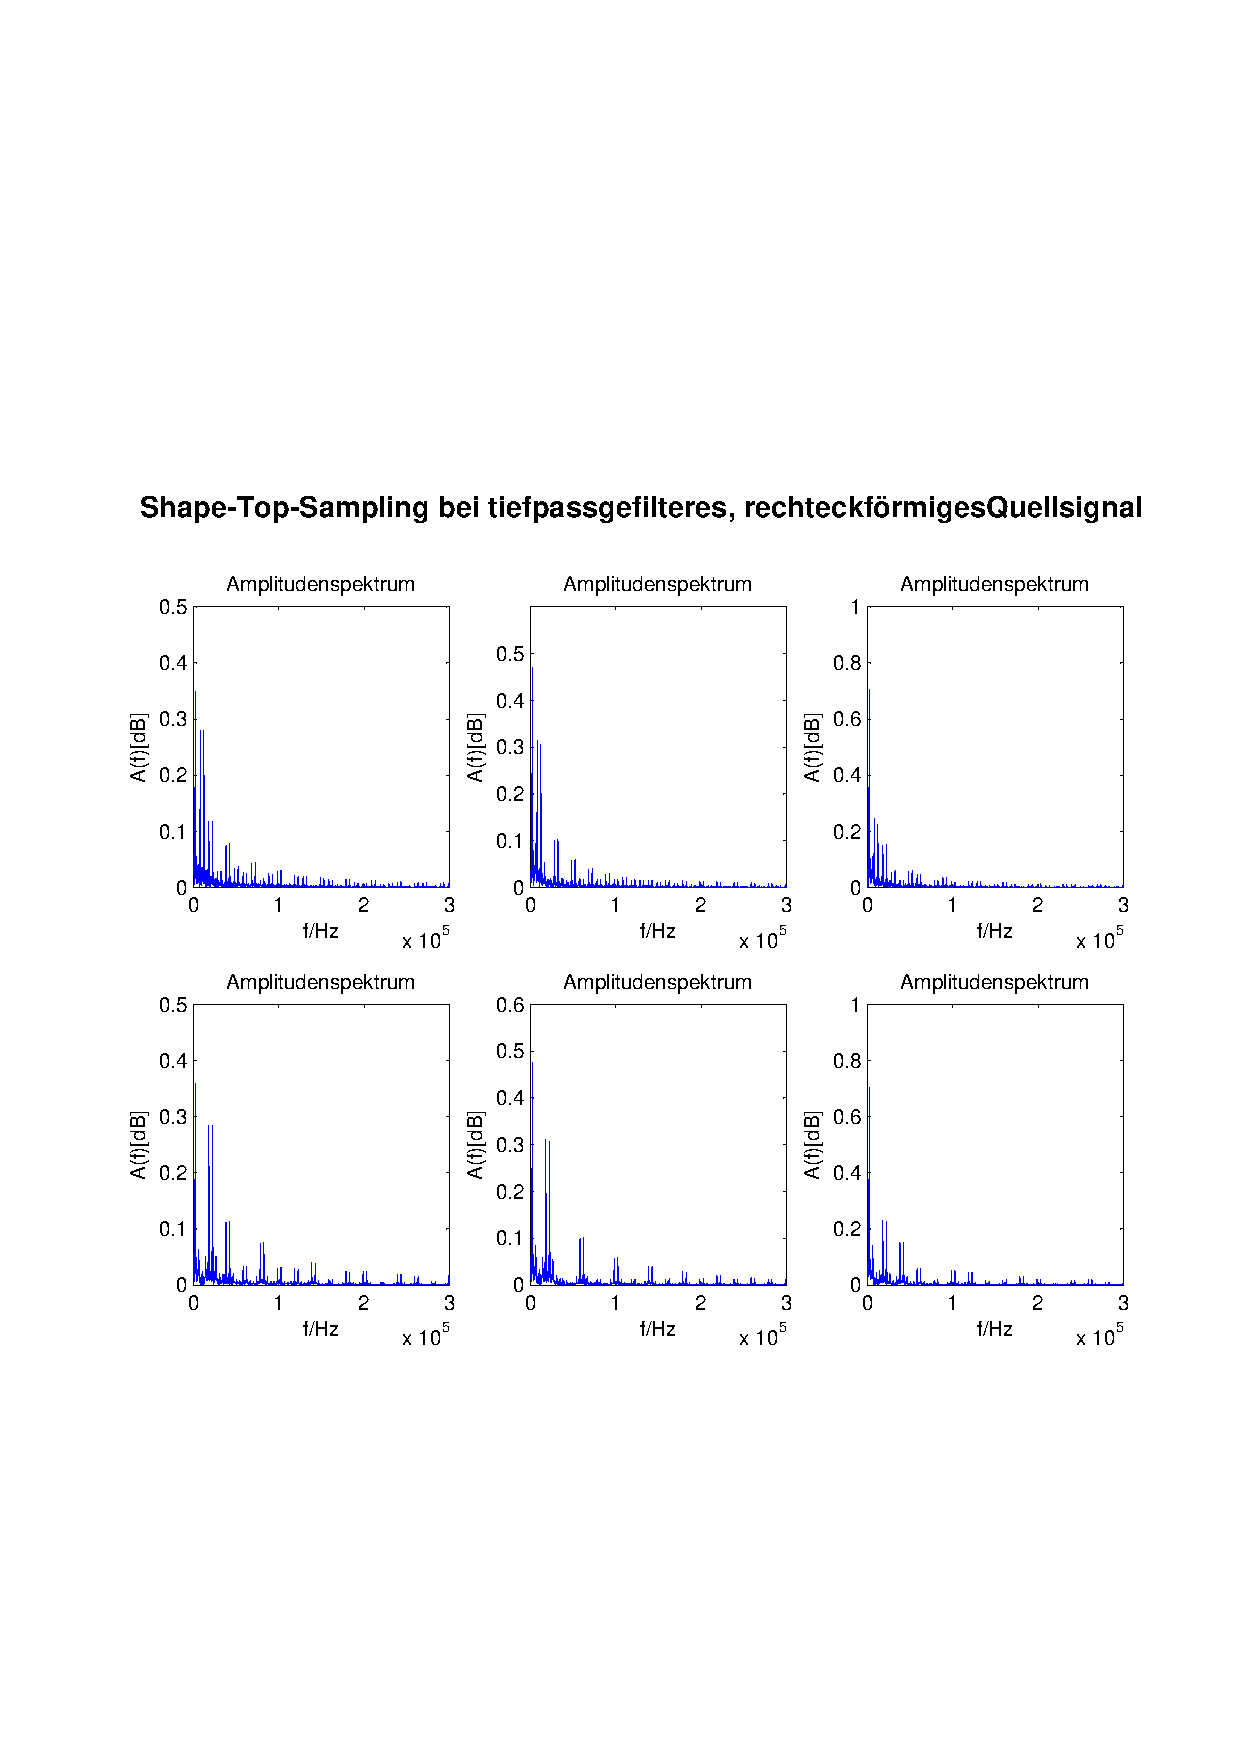
\includegraphics[scale=0.5, trim = 1.5cm 6cm 1cm 8cm,
            clip]{./Bilder/shape-top-tp-recht_freq}
                \caption{Frequenzsignal einer shape-top-sampling eines tiefpassgefilterten Rechteckquellsignals}
      	    \end{figure}
        	
        	Den Erwartungen gemäß, kann man auch hier grob eine si-Funktion
        	erkennen. Typisch für die shape-top Abtastung, besitzen wieder alle
        	Peakpaare die jeweils gleiche Amplitude.
        
        \end{quote}  % Ende Subsection   shape Top  
        
        \subsection{Flat-Top Sampling}
        \begin{quote}
           
           Nun betrachten wir die Ergebnisse einer flat-top Abtastung. Begonnen
           wird wieder mit dem Sinusquellsignal:
           
           \begin{figure}[H]
            \centering
            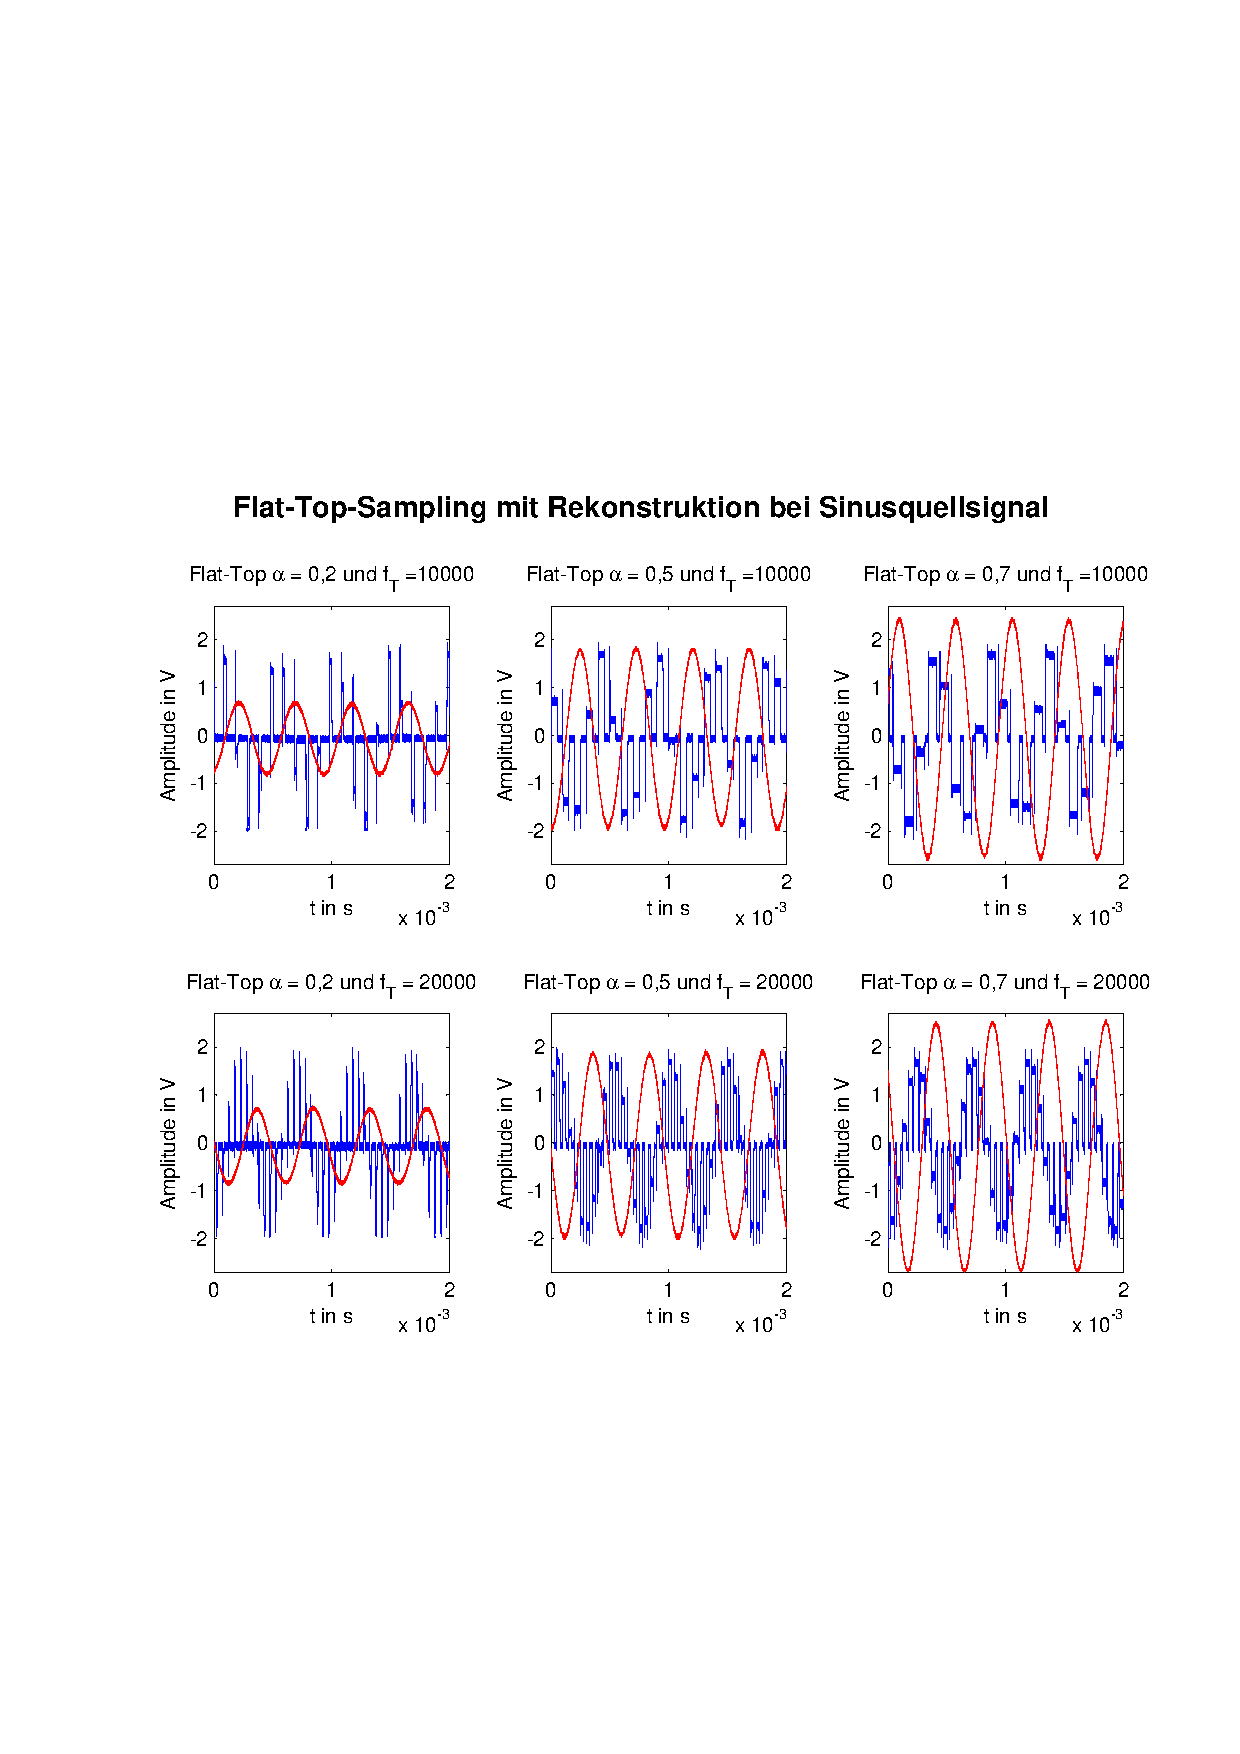
\includegraphics[scale=0.5, trim = 1.5cm 6cm 1cm 8cm,
            clip]{./Bilder/flat-top-sinus}
                \caption{Zeitsignal einer flat-top-sampling mit Rekonstruktion
                eines Sinusquellsignals}
      	    \end{figure}
           
           Wie bei einer flat-top Abtastung erwartet, passen sich die
           Abtastrechtecke nicht dem Sinusverlauf an, sonder nehmen den
           amplitudenwert des Sinus an der Abtaststelle an und behalten diesen
           Wert mithilfe des Sample and Hold Glieds für die gesamte
           Abtastperiode. Daher ist bei einer kleineren Abtastfrequenz ein
           Sinussignal in der modulierten Version kaum erkennbar. Mit einer
           höheren Abtastfrequenz kann man einen Sinusverlauf aber erahnen. Die
           Eigenschaften durch die variable Abtastfrequenz und dem vergrößertem
           $\alpha$ bleiben wie bei der shape-top Abtastung gleich. Die
           Unterschiede in den rekonstruierten Signalen liegen wieder bei den
           Gain- und Grenzfrequenzeinstellungen des verwendeten Tiefpasses.\\
           
           Im Frequenzbereich sieht der flat-top modulierte Sinus folgendermaßen
           aus:
           
           \begin{figure}[H]
            \centering
            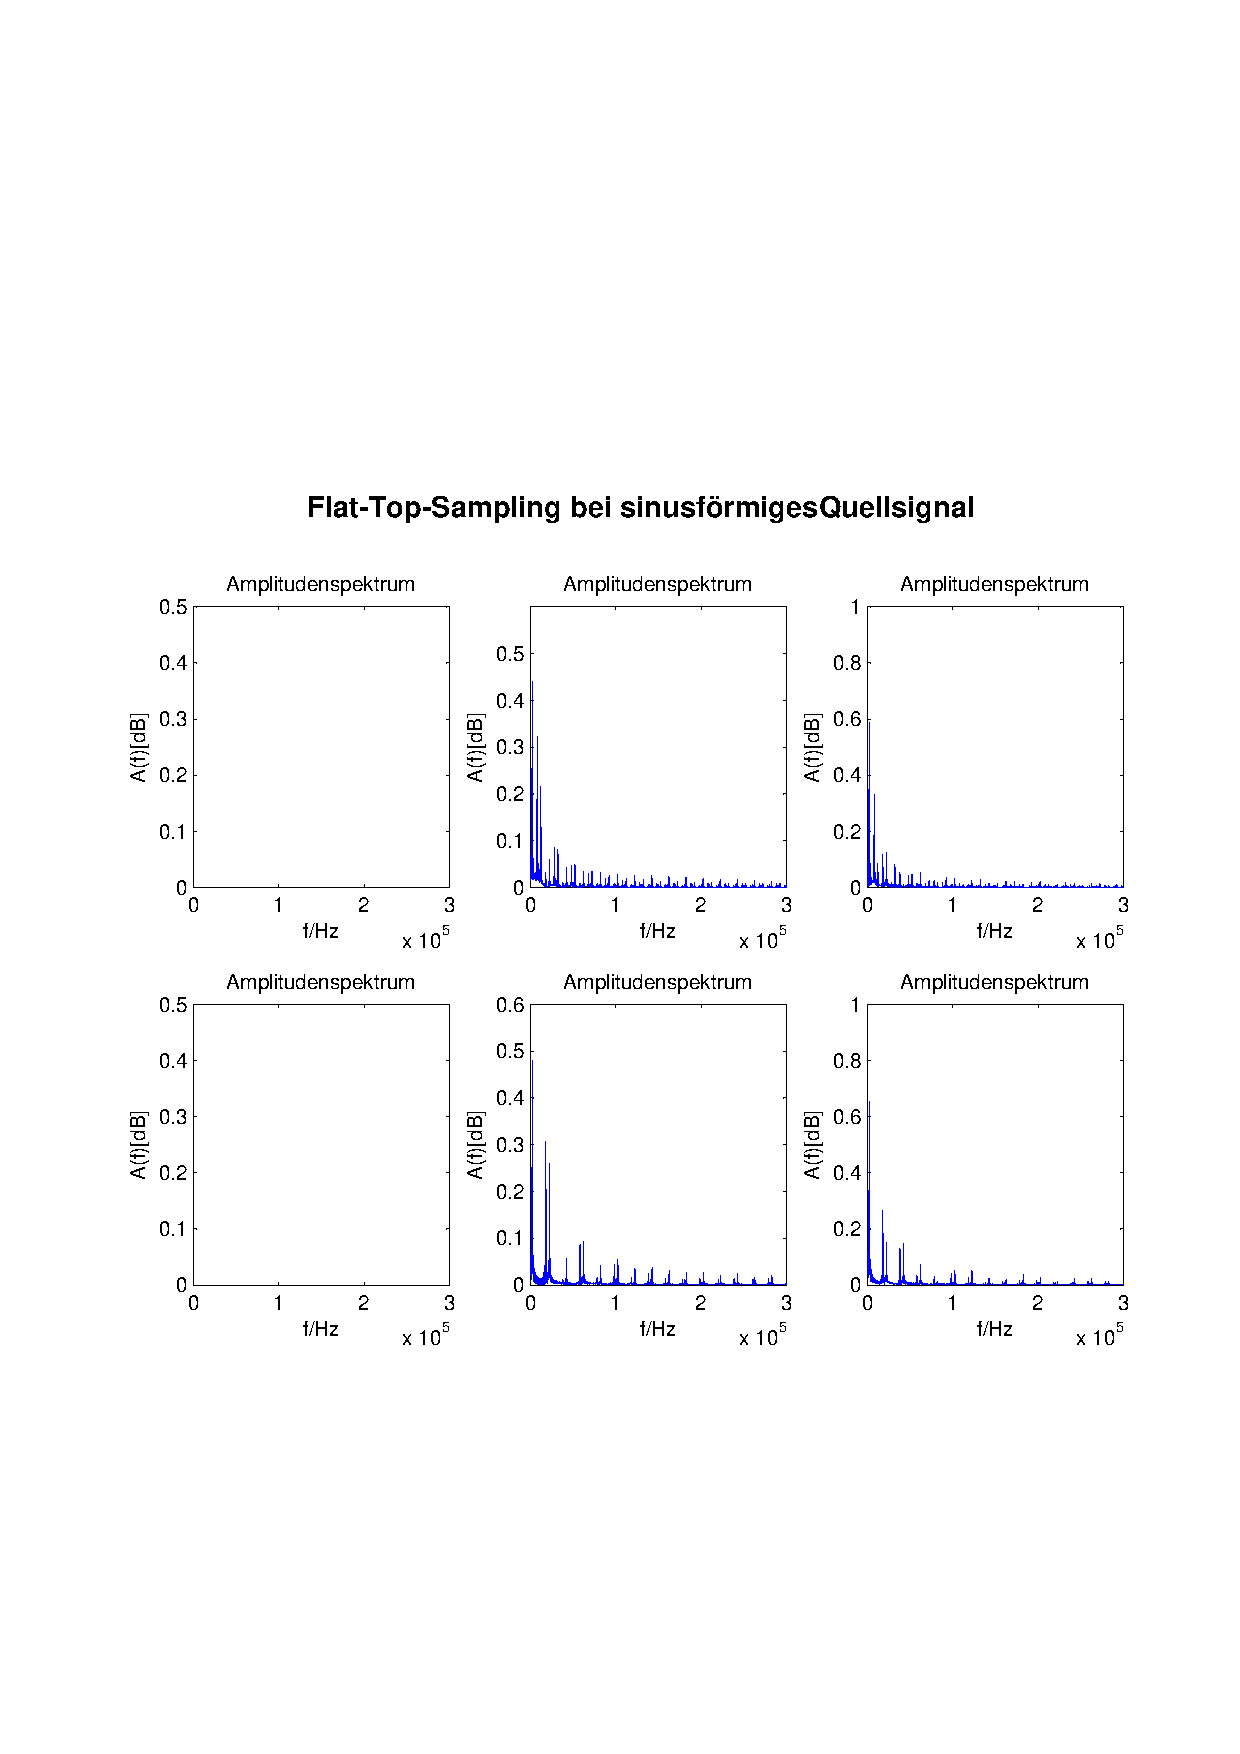
\includegraphics[scale=0.5, trim = 1.5cm 6cm 1cm 8cm,
            clip]{./Bilder/flat-top-sinus_freq}
                \caption{Frequenzsignal einer flat-top-sampling eines Sinusquellsignals}
      	    \end{figure}
           
           Im Vergleich zu den Shape-Top modulierten Signalen lässt sich sehr schön hier die unterschiedlich hohen
           Amplituden eines Bandes erkennen. Auch damit verhält sich unsere Messung wie erwartet und beschrieben.\\
           Auch bei dieser Messung hatten wir zwei Datensätze, die leider kein Spektrum ergaben. Jedoch verhalten sich
           auch hier die restlichen Spektren wie erwartet.
           
           Für ein flat-top moduliertes Rechtecksignal erhalten wir folgende
           Zeitsignale:
           
           \begin{figure}[H]
            \centering
            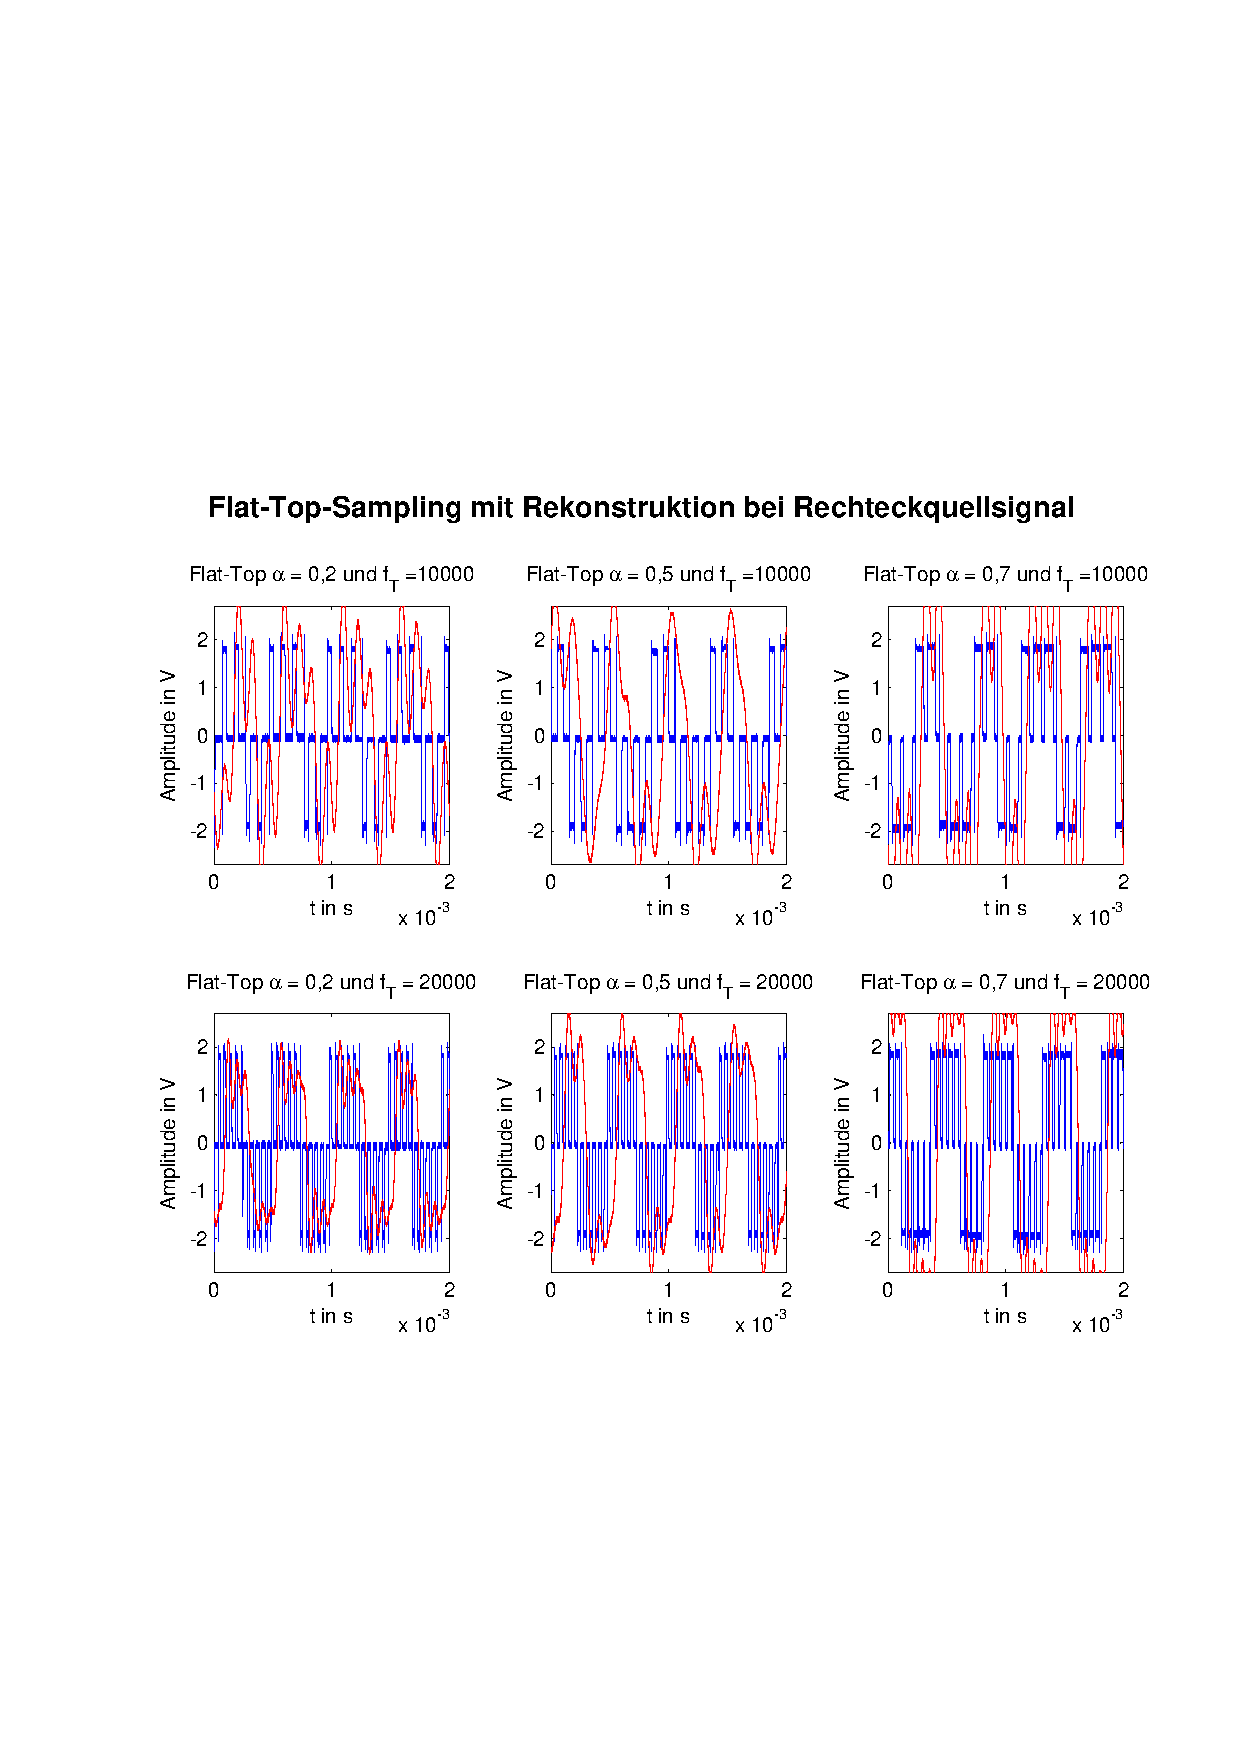
\includegraphics[scale=0.5, trim = 1.5cm 6cm 1cm 8cm,
            clip]{./Bilder/flat-top-recht}
                \caption{Zeitsignal einer flat-top-sampling mit Rekonstruktion
                eines Rechteckquellsignals}
      	    \end{figure}
      	    
      	    Da ein unipolares Rechtecksignal, wie bereits erwähnt, nur aus
      	    entweder einer konstanten Amplitude oder der Amplitude $0 V$ besteht,
      	    ist zwischen einem flat-top und einem shape-top moduliertem
      	    Rechtecksignal kein Unterschied zu sehen, da die Oberflächen der
      	    Abtastrechtecke stets flach sein werden. Dies sieht man auch bei
      	    unseren modulierten Signalen für variable Abtastfrequenzen und
      	    Tastverhältnisse.\\
      	    
      	    Im Frequenzbereich sieht der flat-top modulierte Rechteck wie folgt
      	    aus:
      	    
      	    \begin{figure}[H]
            \centering
            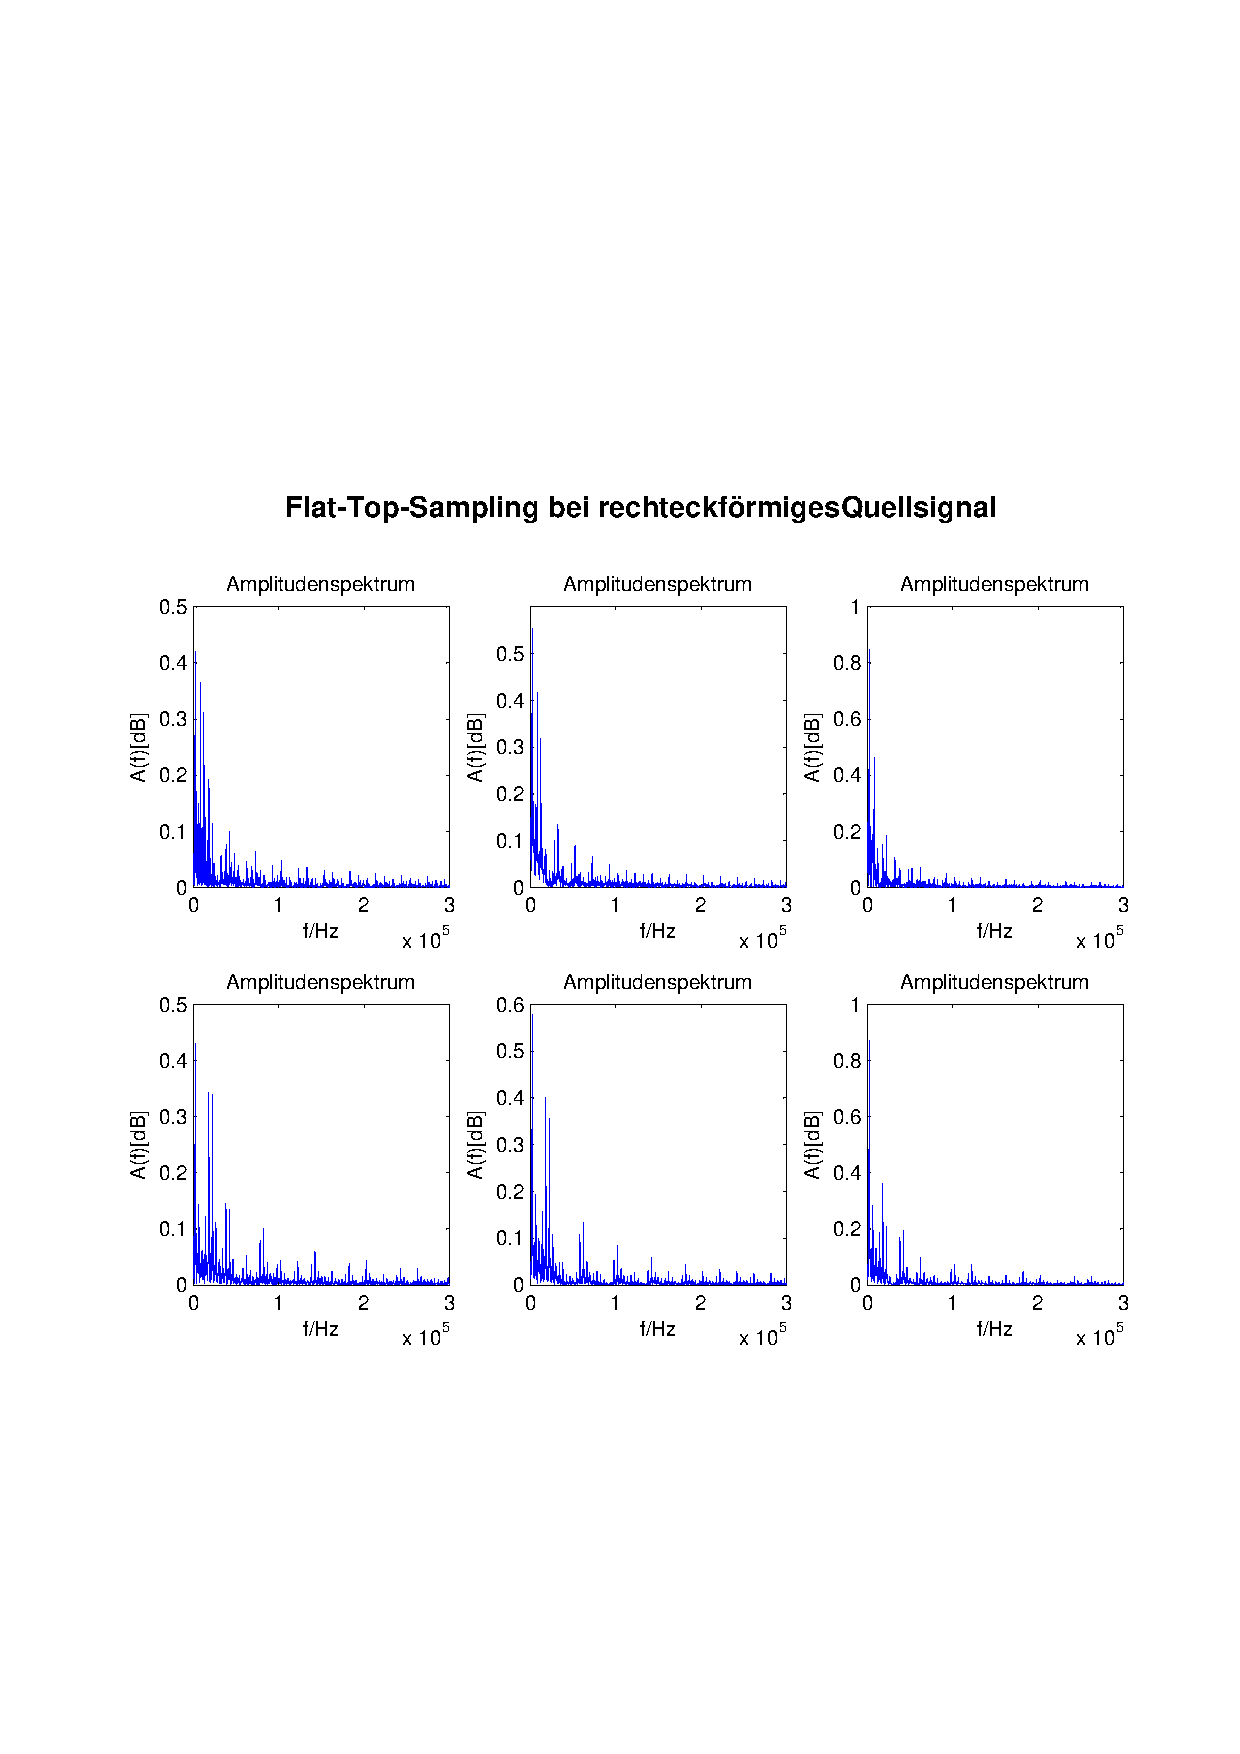
\includegraphics[scale=0.5, trim = 1.5cm 6cm 1cm 8cm,
            clip]{./Bilder/flat-top-recht_freq}
                \caption{Frequenzsignal einer flat-top-sampling eines Rechteckquellsignals}
      	    \end{figure}
      	    
      	    Man kann deutlich erkennen, dass die Peakpaare nicht zwingend die
        	gleiche Amplitude besitzen, wie es beim Spektrum des shape-top sampling
        	der Fall ist. Dadurch, dass die besagten Amplituden bei diesem
        	Abtastverfahren frequenzabhängig sind, wie bereits in der Theorie
        	erklärt, nimmt das Spektrum viel deutlicher den Verlauf einer
        	si-Funktion an.\\
      	    
      	    Zuletzt wird der tiefpassgefilterte Rechteck mit dem flat-top
      	    Verfahren abgetastet und im Zeit- und Frequenzberech untersucht:
      	    
      	    \begin{figure}[H]
            \centering
            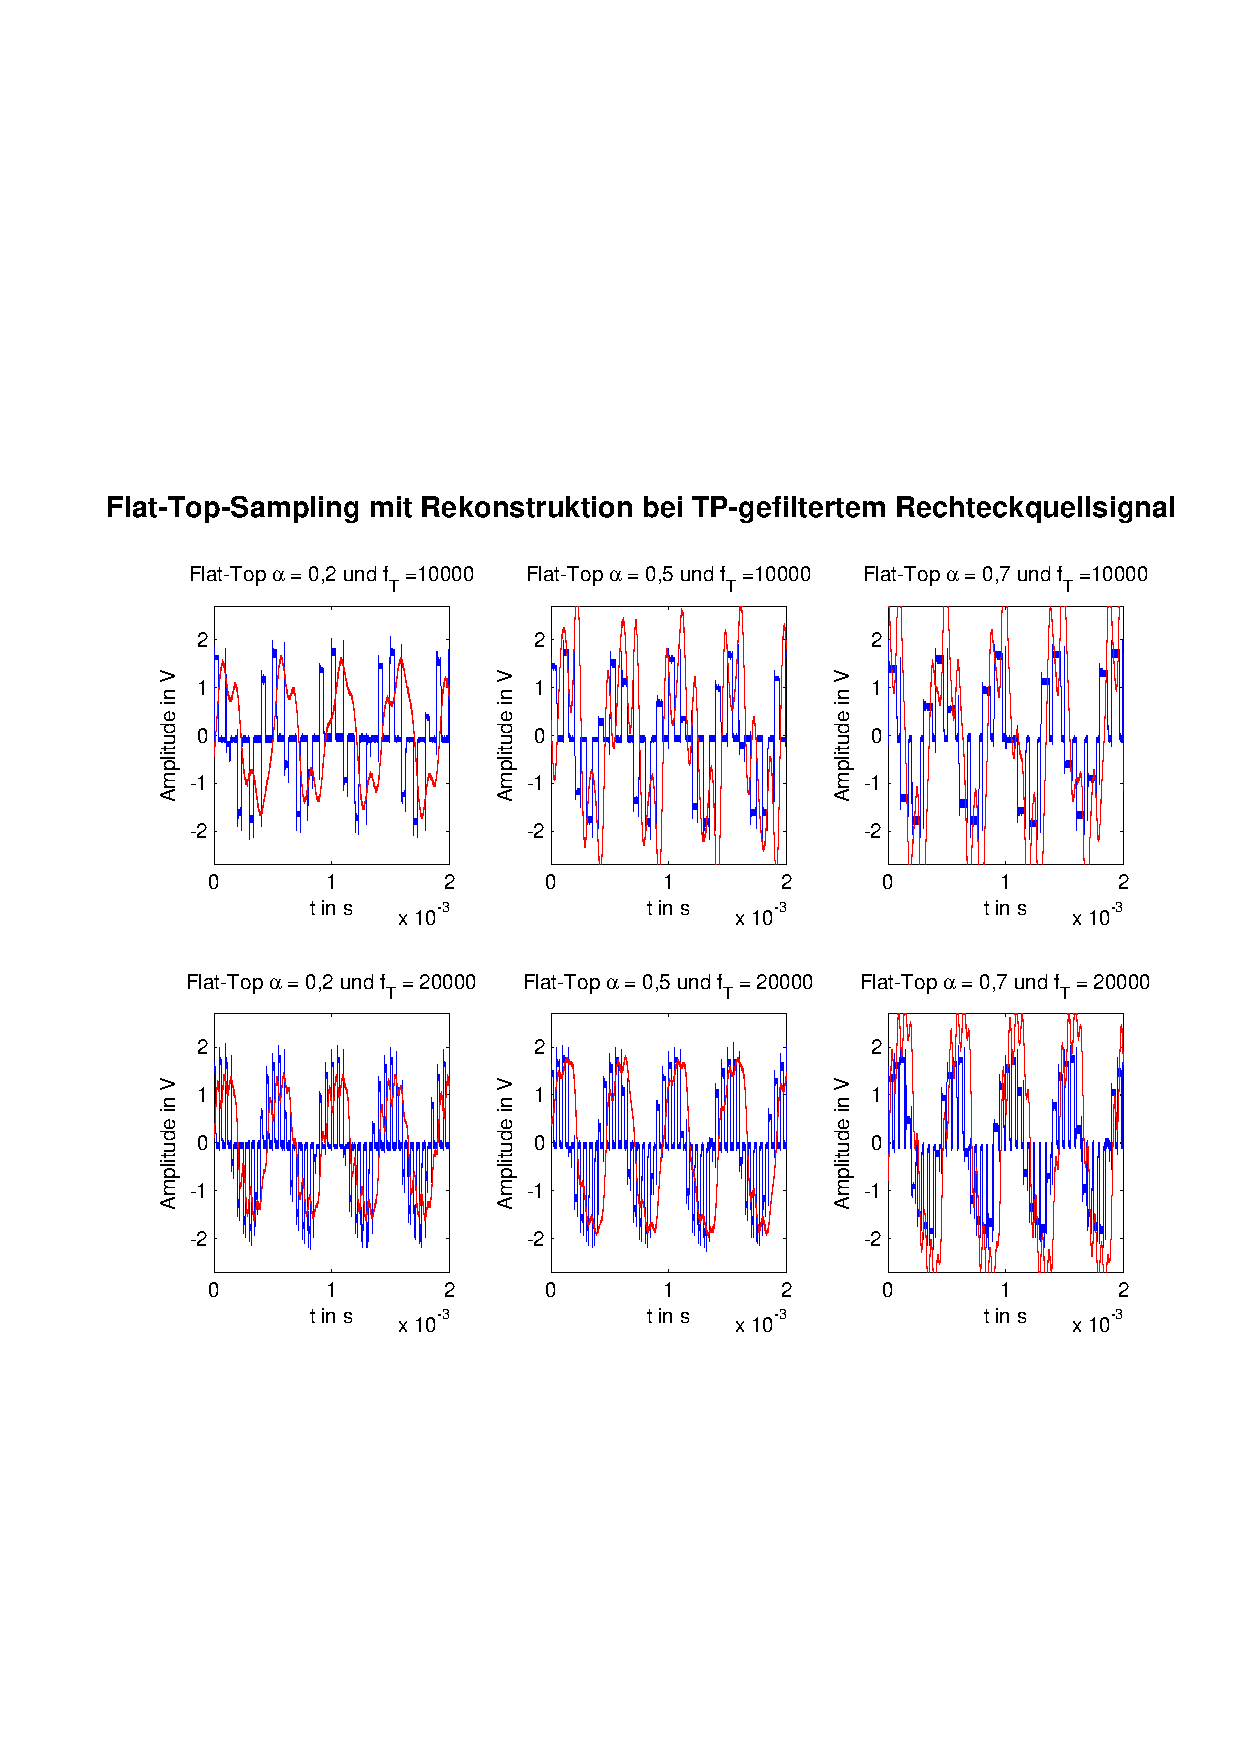
\includegraphics[scale=0.5, trim = 1.5cm 6cm 1cm 8cm,
            clip]{./Bilder/flat-top-tp-recht}
                \caption{Zeitsignal einer flat-top-sampling mit Rekonstruktion
                eines tiefpassgefilterten Rechteckquellsignals}
      	    \end{figure}
      	    
      	    Der tiefpassgefilterte Rechteck hat erneut die gleich Form wie bei
      	    der shape-top Abtastung. Dementsprechend passen sich die flat-top 
      	    Abtastrechtecke dem Quellsignal an und modulieren ihn. Die
      	    Rekonstruktionen sehen bei einer Abtastfreuquenz von $20 kHz$
      	    erneut deutlich besser aus, als bei den $10 kHz$. Dies liegt, wie
      	    bei der shape-top Abtastung bereits erwähnt, an dem Verhältnis
      	    zwischen der im Signal verwendeten Bandbreite und der
      	    Abtastfrequent. Bei der kleineren Abtastfrequenz tritt
      	    Aliasing auf, wodurch die Rekonstruktion verzerrter ist, als bei der
      	    hohen Abtastfrequenz, bei der die mindestens doppelte Bandbreite
      	    gewährleistet ist.\\
      	    
      	    Im Frequenzbereich liefert der tiefpassgefilterte Rechteck folgende
      	    Ergebnisse:
      	    
      	    \begin{figure}[H]
            \centering
            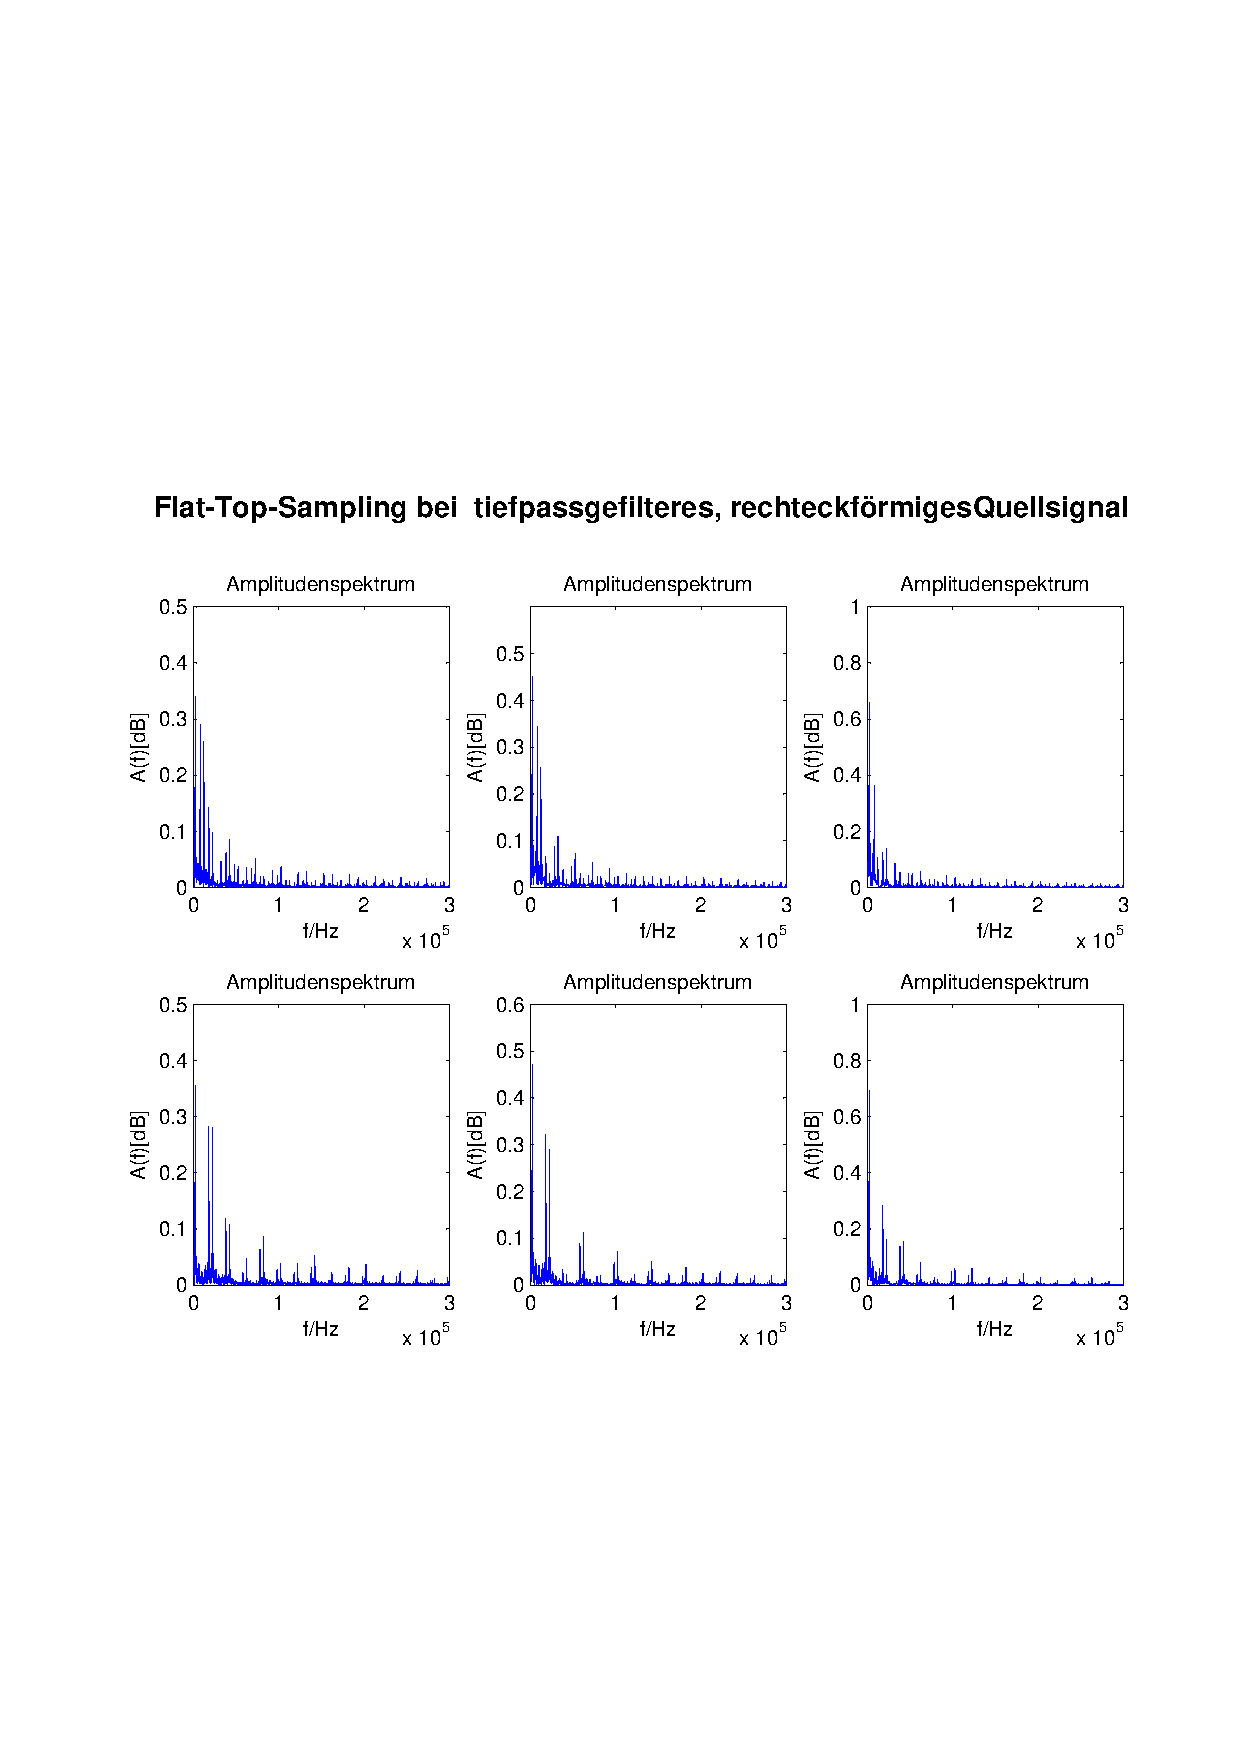
\includegraphics[scale=0.5, trim = 1.5cm 6cm 1cm 8cm,
            clip]{./Bilder/flat-top-tp-recht_freq}
                \caption{Frequenzsignal einer flat-top-sampling eines tiefpassgefilterten Rechteckquellsignals}
      	    \end{figure}
      	    
      	    Ähnlich wie beim Spektrum des flat-top abgetasteten Rechtecksignals,
      	    kann man auch hier ziemlich deutlich den Verlauf einer si-Funktion
      	    erkennen, wodurch sich auch bei dieser Messung unsere Erwartungen
      	    bestätigen.
      	    
        \end{quote}  % Ende Subsection   flat Top    	
       	
       	
       	\newpage
       	
       	\subsection{Sprachsignal}
        \begin{quote}
            Nun werden die Ergebnisse der Sprachübertragung ausgewertet. Zuerst kann
            man die Plots für die aufgenommenen Sprachsignale und ihre Abtastungen
            sehen:
            
            \begin{figure}[H]
            \centering
            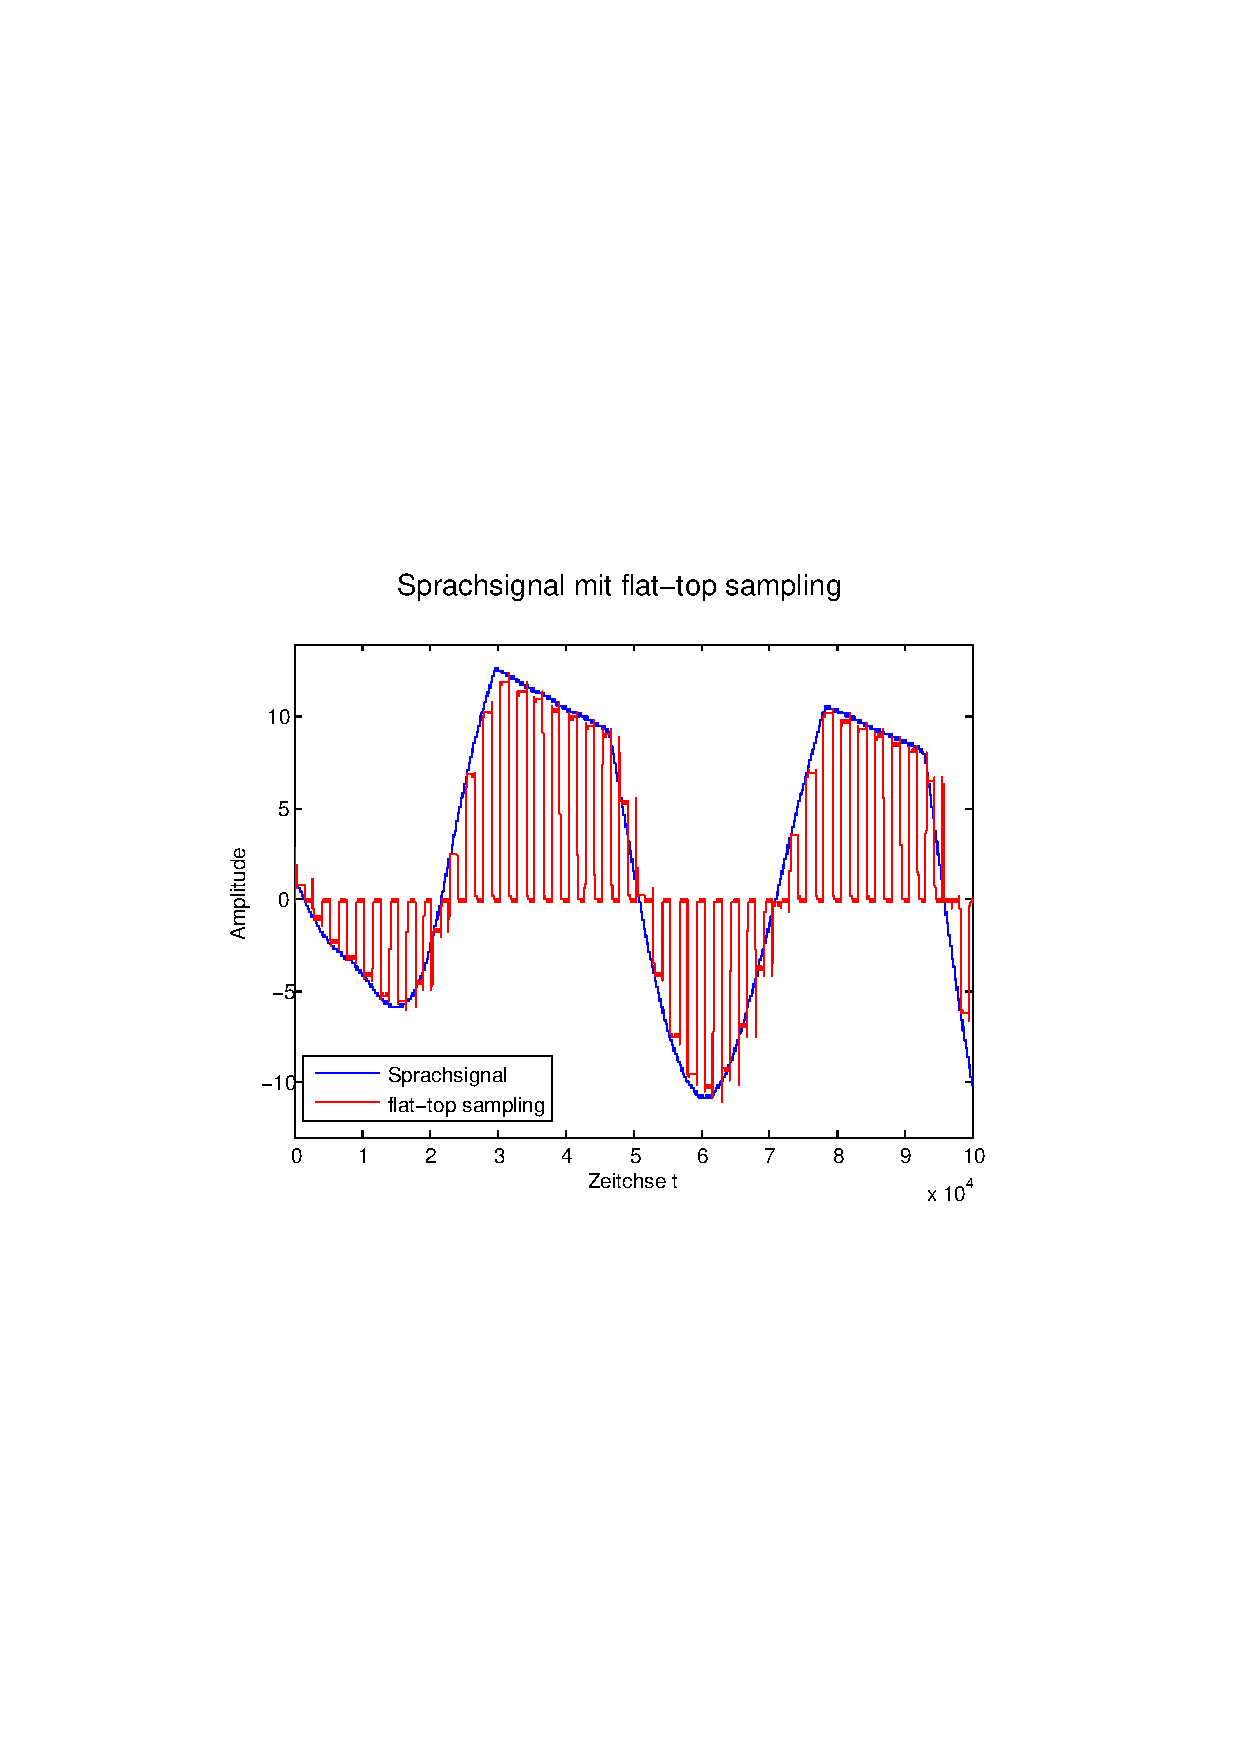
\includegraphics[scale=0.6, trim = 3.5cm 9cm 4cm 9cm,
            clip]{./Bilder/sprache_flat-top}
                \caption{Sprachsignal und die jeweilige flat-top Abtastung}
            \end{figure}
            
            Man kann sehen, dass die flat-top Abtastung auf jeden beliebige Signal
            anwendbar ist. Wie erwartet, nehmen die abtastenden Rechtecke als
            jeweilige Amplitude den Amplitudenwert des Sprachsignals an der
            zeitlichen Position der Abtastung an und behalten diese für die gesamte
            Abtastperiode.\\
            Auch für die shape-top Abtastung ist das Quellsignal nicht relevant:
            
            \begin{figure}[H]
            \centering
            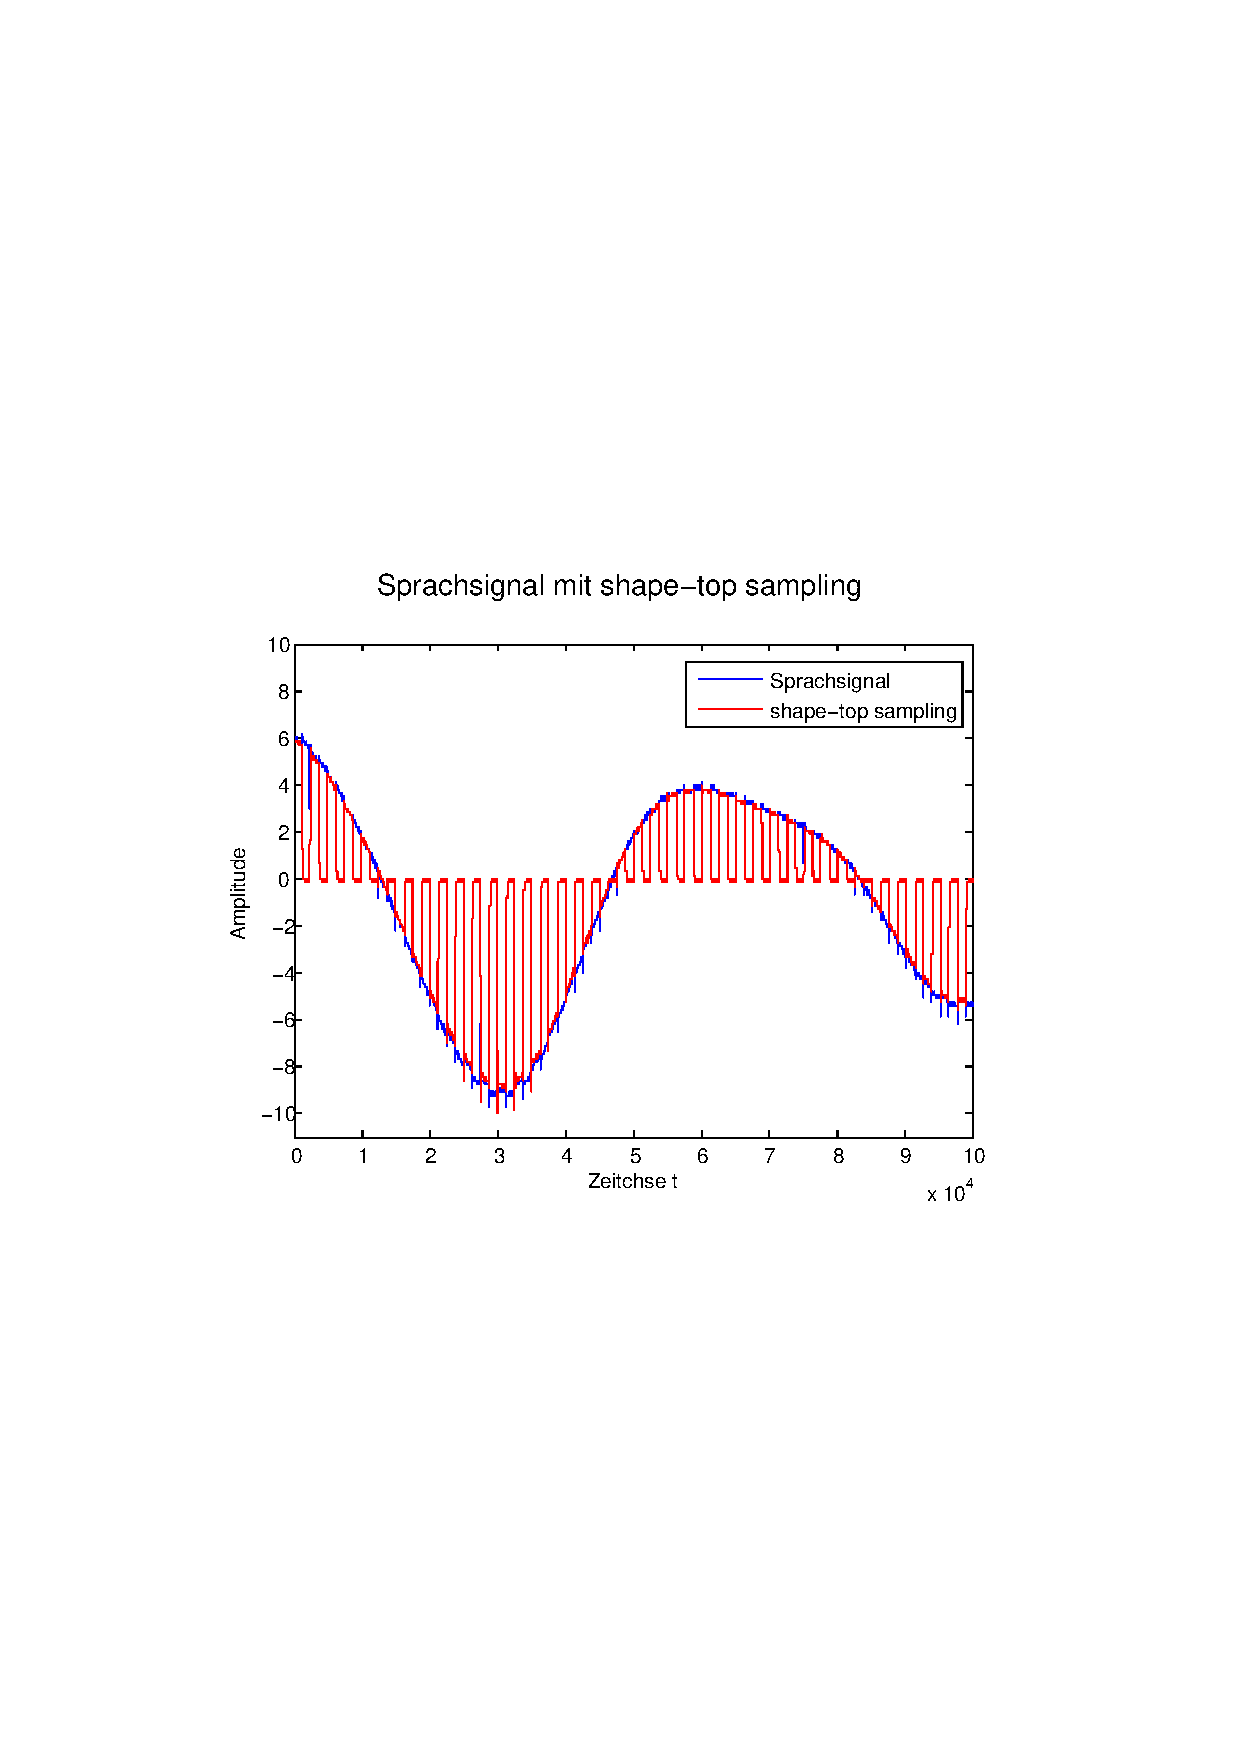
\includegraphics[scale=0.6, trim = 3.5cm 9cm 4cm 9cm,
            clip]{./Bilder/sprache_shape-top}
                \caption{Sprachsignal und die jeweilige shape-top Abtastung}
            \end{figure}
            
            Die Abtastrechtecke nehmen an der Stelle der Abtastung die Amplitude des
            Quellsignals an und verlaufen auch weiterhin, wie beim shape-top
            sampling zu erwarten, über die gesamte Abtastperiode mit der
            Quellsignalamplitude. Beide Abtastsignale bestätigen unsere
            Erwartungen.\\
            
            Zusätzlich wurde ein weiteres beliebiges Sprachsignal aufgezeichnet,
            welches zuerst mit dem flat-top Verfahren abgetastet und später anhand
            eines auf dem Steckbrett vorhandenen Tiefpasses rekonstruiert wurde. Das
            aufgenommene Sprachsignal und die dazugehörige Rekonstruktion ist hier
            zu sehen:
            
            \begin{figure}[H]
            \centering
            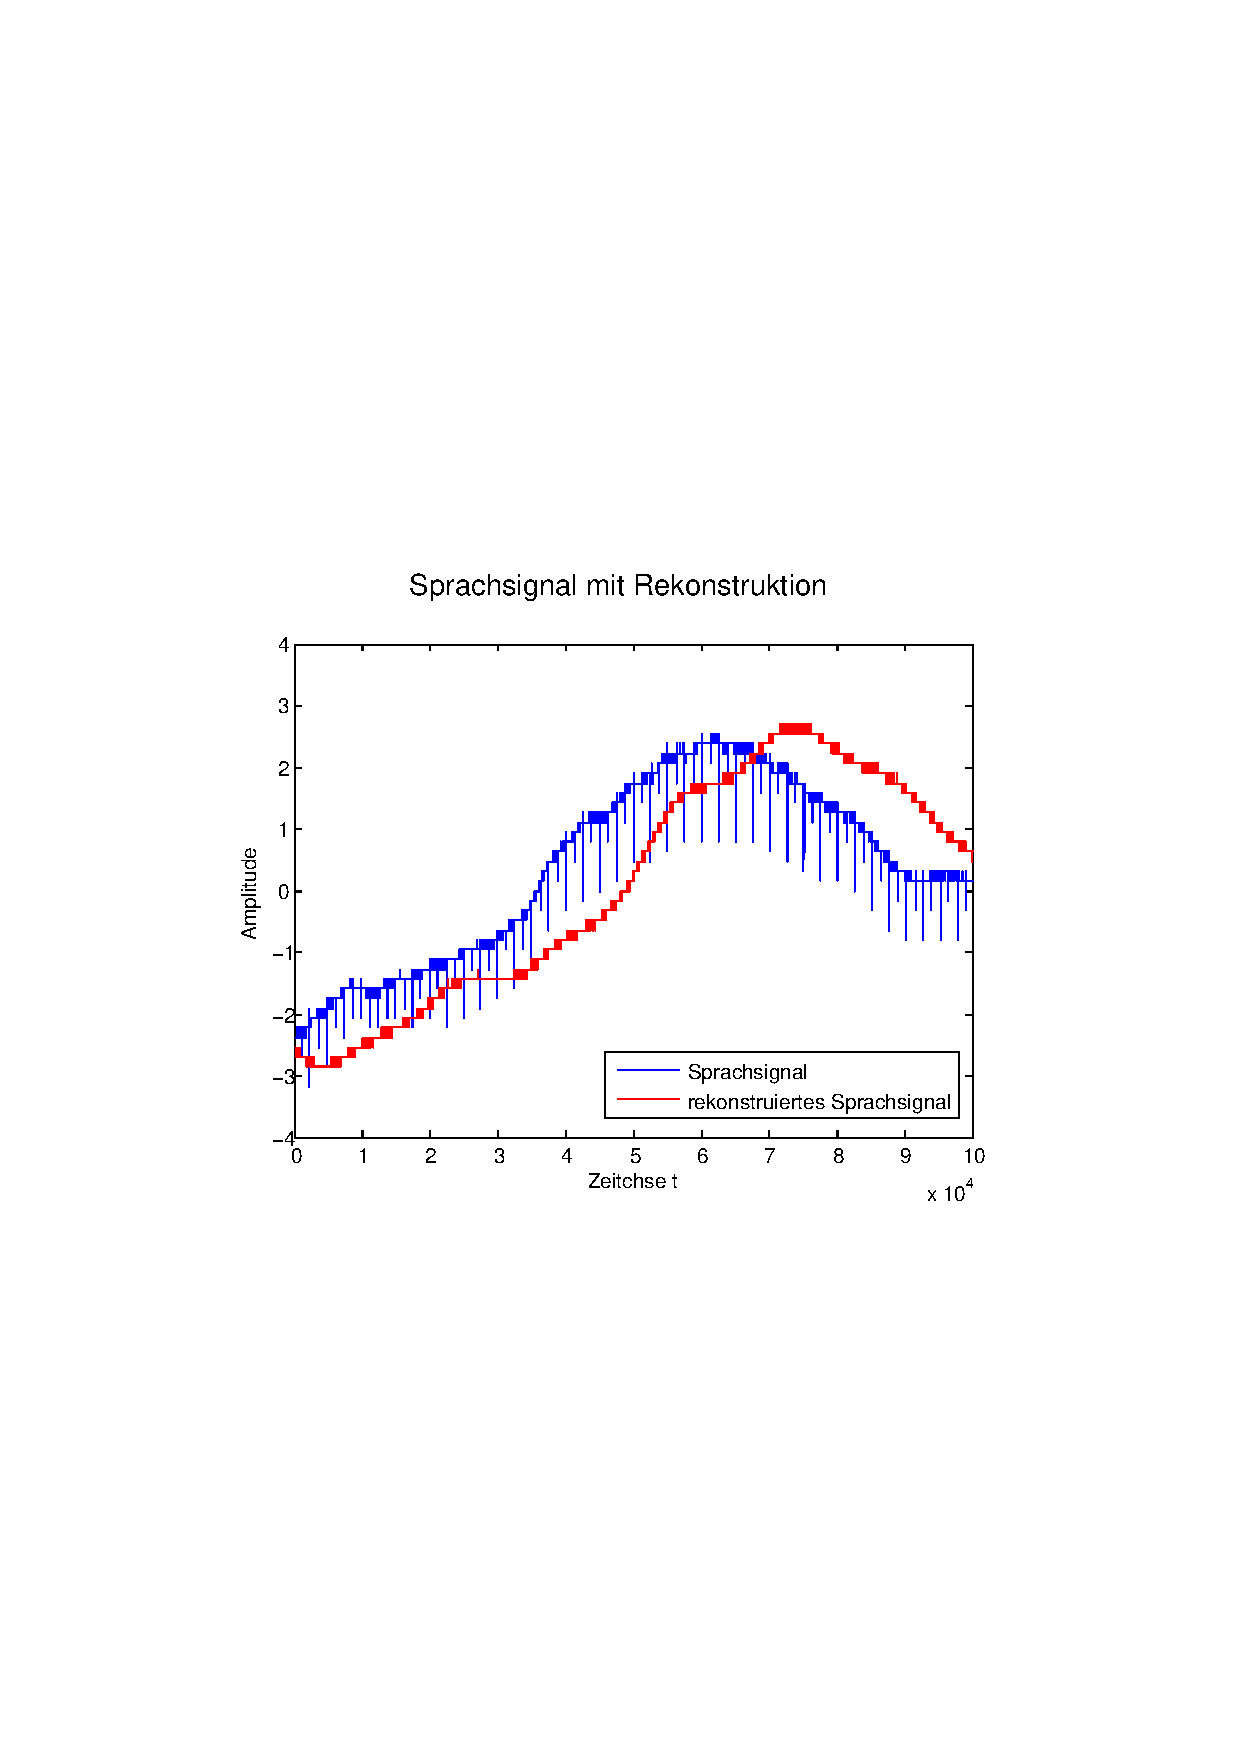
\includegraphics[scale=0.6, trim = 3.5cm 9cm 4cm 9cm,
            clip]{./Bilder/sprache+rekon}
                \caption{Sprachsignal und die jeweilige Rekonstruktion}
            \end{figure}
            
            Auch wenn eine kleine zeitliche Verzögerung vorhanden ist, ist es
            bemerkenswert, wie ähnlich sich das Originalsprachsignal und die
            rekonstruierte Version sind. 
            
            \end{quote}  % Ende Subsection Sprachaufzeichnung
       	
       	
         	
    \end{quote}%beende Auswertung
    
    \section{Zusammenfassung}
    \begin{quote}
	
    	Die praktische Umsetzung der in diesem Praktikum behandelten
    	Pulsamplitudenmodulation bestätigte unsere Erwartungen aus der Theorie. Wir
    	konnten nachvollziehen, wie die beiden Verfahren der Abtastung realisiert
    	werden, indem wir den Aufbau selbstständig ausarbeiteten. Außerdem konnten wir
    	auf dem PicoScope direkt sehen, ob die flat-top bzw. shape-top modulierten
    	Signale im Vergleich zu dem unmodulierten Quellsignal die erwartete Form
    	annahmen. Im Spektrum machten sich dann auch die Vor- und Nachteile der
    	jeweiligen Abtastverfahren erkennbar.
    	
    	\vspace{0.5em}
    	
    	Die Herausforderung in diesem Praktikum bestand hauptsächlich darin, die
    	Schaltung korrekt zu realisieren und die Quellsignale richtig einzustellen.
    	Auch bei den rekonstruierten Signalen mussten wir stets wissen, wie der verwendete 
    	Tiefpass funktioniert und wie jegliche Verstärkungen und Dämpfungen auf dem
    	Steckbrett eingestellt werden mussten.
    	
    	\vspace{0.5em}
    	
    	Die Sprachübertragung war unserer Meinung nach die interessanteste Durchführung
    	im Praktikum, obwohl sich bei dem Aufbau der Schaltung sehr wenig verändert
    	hat. Es war sehr überzeugend zu sehen, dass ein beliebiges Sprachsignal,
    	welches mit einem simplen Mikrofon aufgenommen wurde, so effektiv
    	moduliert und rekonstruiert werden konnte. Wenn man berücksichtigt, dass die
    	zwei behandelten Pulsamplitudenmodulationen die Vorstufe für ein Time-Division-Multiplexing
    	Verfahren sind, dann ist dieses Beispiel sehr realitätsbezogen, da es sich
    	nicht um ein selbsterzeugtes Referenzquellsignal handelt, welches
    	eingesetzt wird, da es einfach zu untersuchen ist, sondern weil es sich um
    	menschliche Sprache handelt, dessen übertragung für die moderne Kommunikation  
    	nicht weg zu denken ist.
	

    \end{quote}%beende Zusammenfassung
         

%--------------------------------------------------------------------
%--------------------------------------------------------------------    


\begin{thebibliography}{999}
 \bibitem {PrinzipSignalausblendung} Prof. Dr.-Ing. Sikora, Thomas; Prof. Dr.-Ing. Noll, Peter: Einführung in die
 Nachrichtenübertragung, S.257
\bibitem {AmplitudenspektrumShap_Top} Prof. Dr.-Ing. Sikora, Thomas; Prof. Dr.-Ing. Noll, Peter: Einführung in die
 Nachrichtenübertragung, S.258
\bibitem {Amplitudenspektrum_Flat_Top} Prof. Dr.-Ing. Sikora, Thomas; Prof. Dr.-Ing. Noll, Peter: Einführung in die
 Nachrichtenübertragung, S.259
 



%Name, Vorname.; evtl. Name2, Vorname2.: Titel des Dokumentes
%oder Buches, Zeitschrift/Verlag/URL (Auflage, Erscheinungsort, -jahr), ggf. Seitenzahlen
% \bibitem {PasevalscheTheorem} \url{https://de.wikipedia.org/wiki/Parsevalsches_Theorem}, Zugriff
% 23.05.2012
\end{thebibliography}

\end{document}
  	    
